\documentclass[14pt]{extarticle}

% --------------------------------------------------
% Encodage et langue
% --------------------------------------------------
\usepackage[utf8]{inputenc}
\usepackage[T1]{fontenc}
\usepackage[french]{babel}
\usepackage{microtype}
\usepackage{xurl}
\usepackage{datetime2}
% Dans le préambule, ajoute si pas déjà présent :
\usepackage{adjustbox}
\usepackage{wrapfig} % dans le préambule
\usepackage[none]{hyphenat}
\binoppenalty=10000
\relpenalty=10000
% --------------------------------------------------
% Mise en page
% --------------------------------------------------
\usepackage[letterpaper,top=2cm,bottom=3cm,left=3cm,right=3cm,marginparwidth=1.75cm]{geometry}
\setlength{\headsep}{40pt}
\usepackage{booktabs}

% --------------------------------------------------
% Mathématiques
% --------------------------------------------------
\usepackage{amsmath,amssymb,amsfonts}
\usepackage{siunitx}

% --------------------------------------------------
% Graphiques & figures
% --------------------------------------------------
\usepackage{graphicx}
\usepackage{subcaption}
\usepackage{tikz}
\usetikzlibrary{arrows.meta, positioning}
\usepackage{pgfplots}
\pgfplotsset{compat=1.18}
\usepackage{float}

% --------------------------------------------------
% Couleurs & liens
% --------------------------------------------------
\usepackage{xcolor}
\definecolor{bleue}{rgb}{0,0,1}
\definecolor{darkgreen}{RGB}{0,100,0}
\usepackage[colorlinks=true, allcolors=bleue]{hyperref}

% --------------------------------------------------
% Table des annexes (personnalisée)
% --------------------------------------------------
\usepackage{tocloft}
\newcommand{\listannexname}{Table des annexes}
\newlistentry{annexe}{loa}{0}
\newcommand{\listofannexes}{\listof{annexe}{\listannexname}}

\makeatletter
\newcommand{\startannexe}[1]{%
  \clearpage
  \refstepcounter{annexe}
  \addcontentsline{loa}{annexe}{Annexe \theannexe\hspace{1em}#1}
  \section*{Annexe \theannexe \quad #1}
}
\makeatother

% --------------------------------------------------
% Autres packages
% --------------------------------------------------
\usepackage[justification=centering, font=footnotesize]{caption}
\usepackage{fancyhdr}
\usepackage{enumitem}
\usepackage{titlesec}

% --------------------------------------------------
% STYLE pages romaines : uniquement numéro de page
% --------------------------------------------------
\fancypagestyle{romain}{
    \fancyhf{}
    \fancyfoot[C]{\thepage}
    \renewcommand{\headrulewidth}{0pt}
    \renewcommand{\footrulewidth}{0pt}
}

% --------------------------------------------------
% STYLE pages corps du rapport : en-tête complet
% --------------------------------------------------
\fancypagestyle{corps}{
    \fancyhf{}
    \fancyhead[L]{\footnotesize \textit{\nouppercase{\leftmark}}}
    \fancyhead[R]{\footnotesize  Epaisseur lors d'une emboutissage en 2 étapes -- Alliage Alu 7075}
    \fancyfoot[C]{\thepage}
    \renewcommand{\headrulewidth}{0.4pt}
    \renewcommand{\footrulewidth}{0.4pt}
}

% pagestyle par défaut = romain (pages préliminaires)
\pagestyle{romain}

\begin{document}

% --------------------------------------------------
% Page de Garde ENSIBS (aucun en-tête)
% --------------------------------------------------
\begin{titlepage}
    \begin{minipage}{0.5\textwidth}
        \begin{flushleft}
            
\includegraphics[width=0.5\textwidth]{Images/LOGO/ensibs-ecole-ingenieurs.jpg}
        \end{flushleft}
    \end{minipage}
    \hfill
    \begin{minipage}{0.4\textwidth}
        \begin{flushright}
            
\includegraphics[width=0.5\textwidth]{Images/LOGO/IRDL.png}
        \end{flushright}
    \end{minipage}

    \vspace{2cm}
    \centering
    \textsc{\Large Rapport de stage de fin d'étude}\\[1cm]

  \rule{\linewidth}{0.8mm}\\[0.3cm]

\begin{center}
{\LARGE \bfseries
Étude expérimentale et numérique de l’évolution de l’épaisseur de la tôle lors de l'opération d’emboutissage à haute température d'un godet cylindrique en alliage d'aluminium AA7075-T6
}
\end{center}

\vspace{0.4cm}
\rule{\linewidth}{0.8mm}\\[2.5cm]

    \begin{minipage}{0.45\textwidth}
        \begin{flushleft} \large
            \emph{Auteur :}\\
            Sena \textsc{Razafy}
        \end{flushleft}
    \end{minipage}
    \hfill
    \begin{minipage}{0.45\textwidth}
        \begin{flushright} \large
            \emph{Encadrants :}\\
            Hervé \textsc{Laurent}\\
            Constant \textsc{Ramard}
        \end{flushright}
    \end{minipage}

    \vfill
    {\large Promotion 2026}\\[0.5cm]
    {\large \ Spécialité Mécatronique}\\[0.5cm]
\end{titlepage}

% --------------------------------------------------
% Pages préliminaires — style ROMAIN (sans en-tête)
% --------------------------------------------------
\newpage
\pagenumbering{roman}
\pagestyle{romain}

\begingroup
\hypersetup{linkcolor=black}
\tableofcontents
\newpage
\listoffigures
\endgroup
\newpage
\listoftables

% --------------------------------------------------
% Résumé / Abstract — style ROMAIN (sans en-tête)
% --------------------------------------------------
\newpage
\section*{Résumé / Abstract}
\addcontentsline{toc}{section}{Résumé / Abstract}

\textbf{Français}\\[0.4cm]
\noindent
[Résumé en français à rédiger.]

\vspace{0.5cm}
\noindent\textbf{Mots-clés :} 

\vspace{1.5cm}

\textbf{English}\\[0.4cm]
\noindent
[Abstract to be written.]

\vspace{0.5cm}
\noindent\textbf{Keywords:} 

% --------------------------------------------------
% Corps du rapport — style CORPS (avec en-tête complet)
% --------------------------------------------------
\newpage
\pagenumbering{arabic}
\setcounter{page}{1}
\pagestyle{corps}            % ← EN-TÊTE ACTIVÉ ICI SEULEMENT

\section{Introduction}
(A Compléter)
%La réduction des gaz à effets de serre est devenu un problématique incoutournable pour tous les secteurs industriels. Dans ce domaine, plus de 90 pourcent de ces émissions proviennent de l'industrie de transport \cite{royne_etude_2025}.

% Ton contenu ici

% --------------------------------------------------
\newpage  % ← saute à la nouvelle page
\section{Matériels et Méthodes}
Pour ce faire, les profils des godets ont été mesurés expérimentalement, puis comparés aux résultats d’une simulation numérique d’emboutissage.
L’objectif de cette étude est de déterminer l’épaisseur des deux godets, présentés dans la section suivante (titre), emboutis en 2 étapes successives réalisées au cours  de la thèse de S.Royne \cite{royne_etude_2025}. 
%selon les profils en directions DL(Direction de Laminage), DT(Direction Transverse) et DD(Direction Diagonale) de la tôle initiale.
%Nous nous sommes basés sur la méthodologie qui existe dans les états de l'art comme celui de \cite{coer_mise_nodate}, \cite{lanterne_local_nodate}, \cite{bazylevych_procedure_2008}  qui ont utilisé les profils des points intérieurs et extérieurs de la pièce pour en déduire l'épaisseur réelle. 
Comme classiquement utilisé dans la littérature \cite{coer_mise_nodate}, \cite{lanterne_local_nodate}, \cite{bazylevych_procedure_2008}, l'épaisseur est obtenue à partir des profils intérieurs et extérieurs des godets suivant 3 directions, la DL, la DT et la DD de la tôle initiale.

\subsection{Présentation des deux étapes d'emboutissage}
Deux types de godets obtenus à l’issue de deux opérations successives d’emboutissage ont été étudiés à partir des travaux de S. Royne \cite{royne_etude_2025}.
Le premier godet, dont les dimensions sont présentées à la figure~\ref{fig:Step1Emboutissage}, est réalisé lors de la première étape d’emboutissage (Step 1) à l’aide des outils illustrés à la figure~\ref{fig:OutilsStep1}. La pièce est formée à partir d’une tôle plane circulaire, communément appelée flan, de diamètre initial 157mm et d’épaisseur e=0,8mm.
Après cette première passe, on remet le premier godet formé sur un autre outil sur la figure~\ref{fig:Step2Emboutissage}, pour être de nouveau embouti afin d'obtenir la forme finale illustrée sur la figure~\ref{fig:OutilsStep2}. Ces deux étapes sont résumées à travers la figure~\ref{fig:StepsEmboutissage} venant de la thèse de S.Royne \cite{royne_etude_2025}. Au début de ces deux étapes, le flan est chauffé à différentes températures selon des cas étudiés, mais pour notre étude, on ne prend en compte que les godets emboutis à une température de 200 °C, car c'est la condition qui semble être la plus optimale pour l'emboutissage de l'alliage alu 7075 selon S.Royne \cite{royne_etude_2025}. Par ailleurs, l’effort de serrage appliqué entre le serre-flan et la matrice n’est imposé qu’au cours de la première étape d’emboutissage. Deux niveaux d’effort ont été étudiés : CF1=41kN et CF2=66kN.


%Debut figure
\begin{figure}[H]
    \centering

    % -----------------------------------------------
    % LIGNE 1 : Photos des outils/procédé
    % -----------------------------------------------
    \begin{subfigure}[t]{0.45\textwidth}
        \centering
        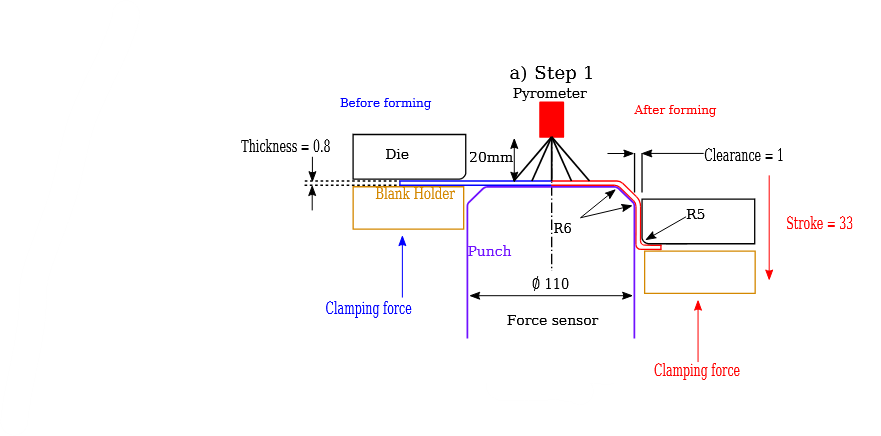
\includegraphics[width=\textwidth]
            {FiguresALL/Methodologie/outils_embouti_1.png}
        \caption{Procédé d'emboutissage pour l'étape 1}
        \label{fig:OutilsStep1}
    \end{subfigure}
    \hfill
    \begin{subfigure}[t]{0.45\textwidth}
        \centering
        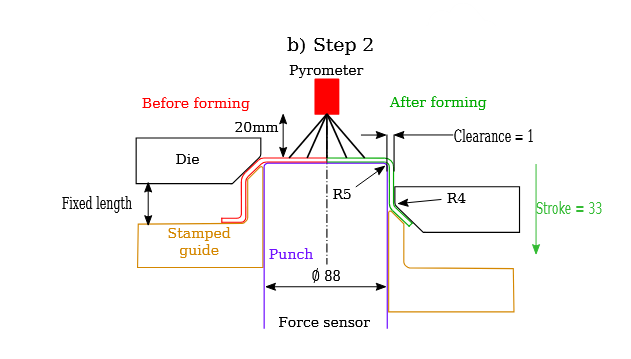
\includegraphics[width=\textwidth]
            {FiguresALL/Methodologie/outils_embouti_2.png}
        \caption{Procédé d'emboutissage pour l'étape 2}
        \label{fig:OutilsStep2}
    \end{subfigure}

    \vspace{0.4cm} % Espace entre les deux lignes

    % -----------------------------------------------
    % LIGNE 2 : Godets obtenus après chaque étape
    % -----------------------------------------------
    \begin{subfigure}[t]{0.45\textwidth}
        \centering
        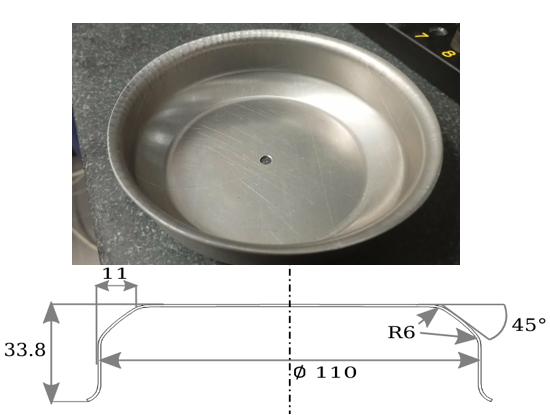
\includegraphics[width=\textwidth, height=5.5cm, keepaspectratio]
            {FiguresALL/Methodologie/Step1Emboutissage.png}
        \caption{Godet intermédiaire obtenu après l'étape 1}
        \label{fig:Step1Emboutissage}
    \end{subfigure}
    \hfill
    \begin{subfigure}[t]{0.45\textwidth}
        \centering
        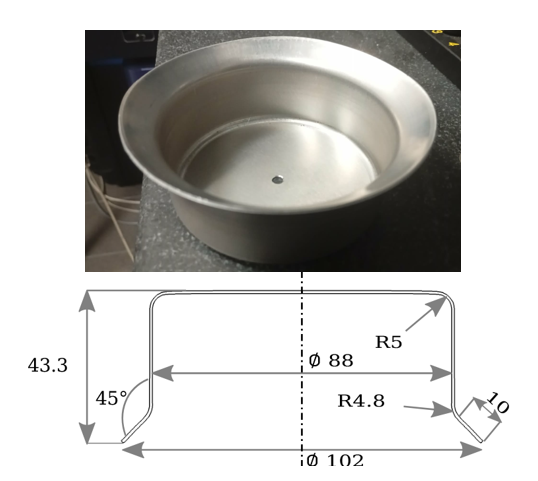
\includegraphics[width=0.85\textwidth, height=5.5cm, keepaspectratio]
            {FiguresALL/Methodologie/STEP2emboutissage.png}
        \caption{Forme finale du godet obtenue après l'étape 2}
        \label{fig:Step2Emboutissage}
    \end{subfigure}

    \caption{Les deux étapes d'emboutissage successives permettant d'obtenir
             le godet cylindrique final en alliage AA7075 : (a)(b) mise en
             position des outils, (c)(d) godets résultants.}
    \label{fig:StepsEmboutissage}
\end{figure}
%fin figure


% --------------------------------------------------
%Première section là on explique l'expérimental le fait de comment on fait réellement pour mesurer l'évolution de l'épaisseur avec quel moyen quel outil et tout avec des bibliographies parlant
\subsection{Protocole de mesure expérimentale des profils des godets}
Pour obtenir les profils intérieur et extérieur des  godets expérimentals, un palpage discret de points le long des directions du godet a été réalisé.
Dans un premier temps, les directions DL, DD et DT du godet sélectionné pour les mesures sont repérées sur le fond extérieur de la pièce. Ce marquage permet à la fois de distinguer les différents profils étudiés et de faciliter le repositionnement du godet lors des opérations de mesure ultérieures.

%Contenu






%-----------------Version__Old--------
%Deux types de godets, présentés à la figure~\ref{fig:StepsEmboutissage}, et obtenus lors des deux étapes d’emboutissage décrites dans l'article de \cite{royne_etude_2025}, sont repris dans cette partie. L’objectif est de mesurer les profils intérieur et extérieur à l’aide d’un palpage discret de points le long des surfaces. Les godets emboutis avec une température à 200°C sont les premiers concernés pour cette expérience de mesure car c'est la condition qui semble être la plus optimale pour l'emboutissage de l'alliage alu 7075 selon \cite{royne_etude_2025}. Les directions de laminage des godets choisis sont marqués sur le fond extérieur du godet pour faciliter la mise en position de ce dernier ultérieurement. 
%Ces outils cités ci-dessous étaient indispensable pour bien mener ces expériences de palpage de profil de godets. 
Une machine tridimensionnelle (MMT) de la marque Mitutoyo, modèle CRYSTA‑Apex S 544, présentée dans la Figure~\ref{fig:MMT} était utilisée pour faire ce palpage de profil. 
Cette machine est équipée d’un système de déplacement selon trois axes ($\vec{x}$,  $\vec{y}$,  $\vec{z}$) permettant de positionner une tête de palpage sur une zone définie. Cette machine a un palpeur qui est composé d'une tige de 40 mm et une bille de rubis de diamètre 2mm ce qui permet d' obtenir une précision de mesure de l'ordre du micromètre selon l'article \cite{manlay_machines_nodate}. 


%Bloc figure modèle
\begin{figure}[H]                          % [H] = figure exactement ICI dans le texte
    \centering                             % centrage de l'image
    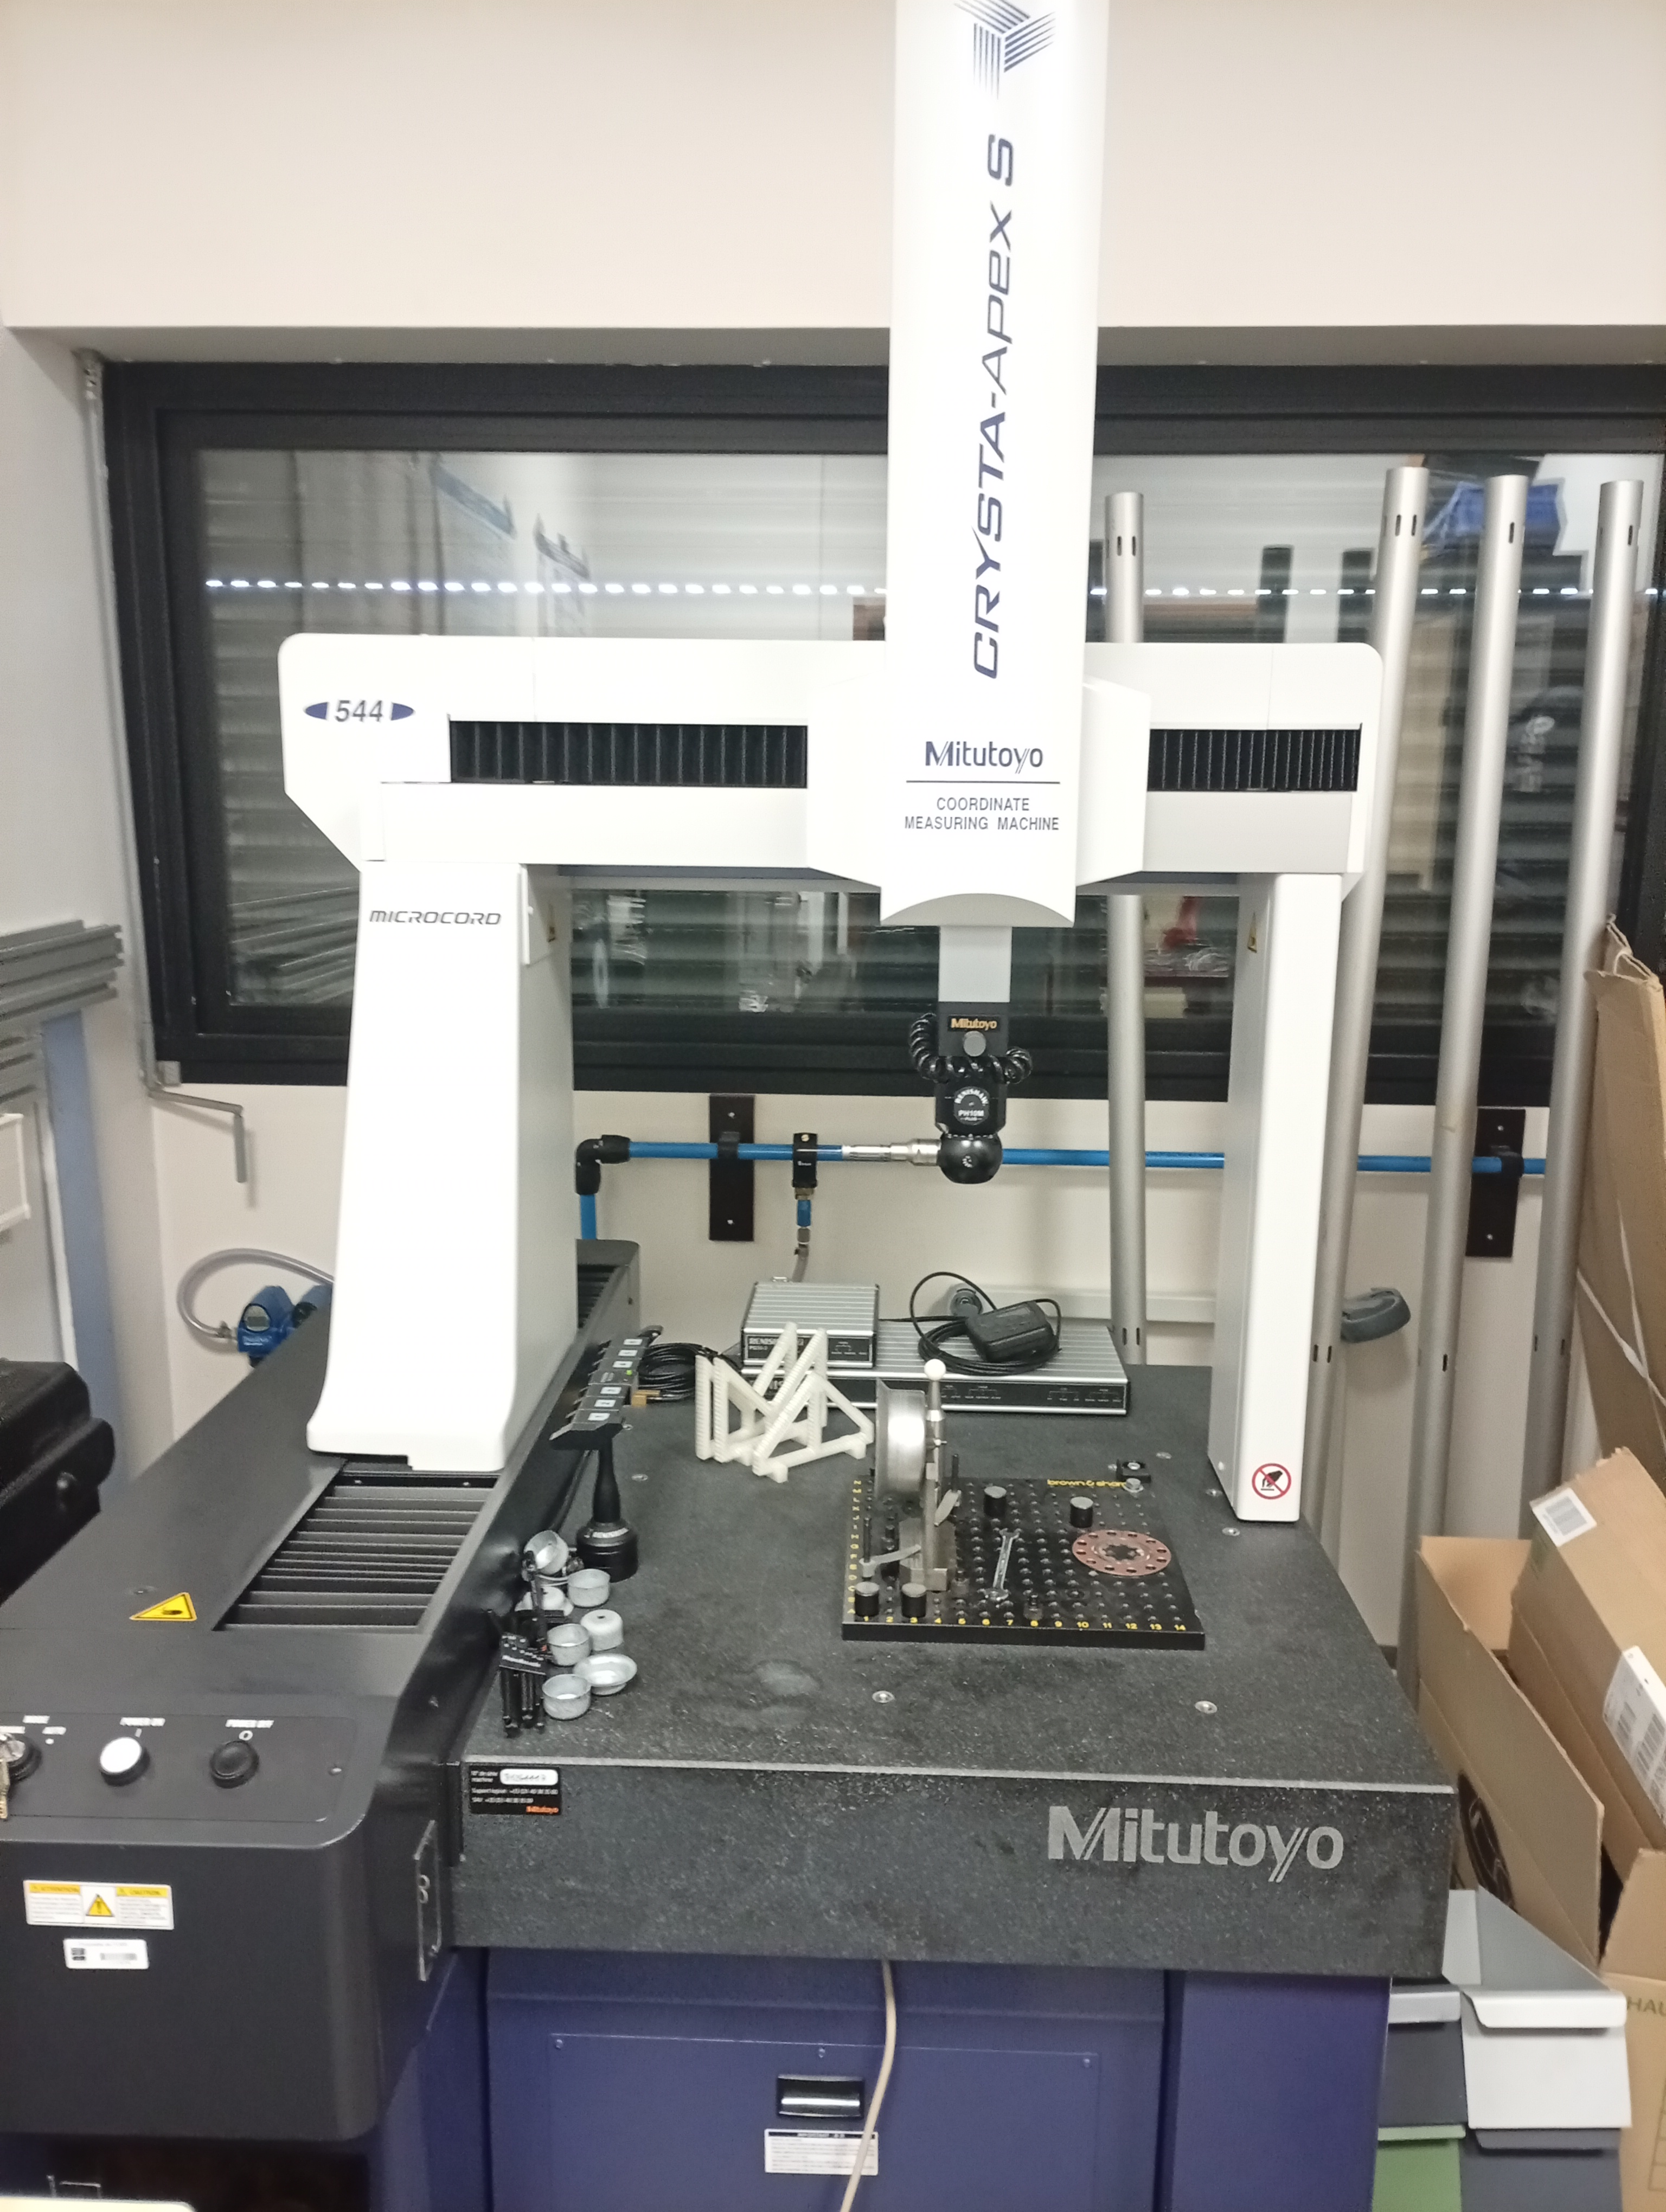
\includegraphics[width=0.4\textwidth]{FiguresALL/Methodologie/MMT4.jpg}  % chemin + taille
    \caption{Machine à mesure tridimensionnelle, Mitutoyo, modèle CRYSTA‑Apex S 544}   % légende affichée sous l'image
    \label{fig:MMT}                  % étiquette pour rappeler la figure
\end{figure}
%fin figure
Dans un premier temps, un perçage centré est réalisé au niveau du godet à l’aide d’un gabarit dédié, développé dans le cadre des travaux de \cite{royne_etude_2025}. Comme illustré à la figure~\ref{fig:MethodePerçage}, ce dispositif permet de maintenir le godet par ses extrémités tout en guidant la mèche, afin de garantir un perçage coaxial à l’axe de révolution de la pièce.

Une fois le godet percé, celui-ci est monté sur le support de métrologie présenté à la figure~\ref{fig:fixationGodet}. Ce support, développé dans le cadre des travaux de J.Coër\cite{coer_mise_nodate}, permet le positionnement du godet lors des essais de mesure et assure le déplacement du palpeur de la MMT le long des différents profils de la pièce.

La fixation entre le godet et le support est réalisée au niveau de la zone centrale du godet à l’aide d’une vis CHC M5 traversante, associée à un écrou. Enfin, le godet est orienté par rapport à la traverse du support de manière à faire coïncider le profil mesuré avec la direction de laminage (DL).





%Le support de métrologie, illustré à la figure~\ref{fig:fixationGodet}, est utilisé pour positionner les godets lors des essais de mesure, permettant le déplacement du palpeur le long de chaque profil. Ce dispositif a été développé dans le cadre des travaux de \cite{coer_mise_nodate}.

%En amont du montage, un perçage centré du godet est réalisé à l’aide d’un gabarit dédié, conçu dans le cadre des travaux de \cite{royne_etude_2025}. Comme illustré à la figure~\ref{fig:MethodePerçage}, cet outil permet de maintenir le godet par ses extrémités tout en guidant la mèche, garantissant ainsi un perçage coaxial à l’axe de révolution.

%La fixation entre le support et le godet est réalisée au niveau de la zone centrale de ce dernier, à l’aide d’une vis CHC M5  traversante et d’un écrou. Le godet est ensuite orienté par rapport à la traverse du support, de manière à coïncider avec le profil suivant la direction de laminage (DL).
%-Un support de métrologie montré par la figure~\ref{fig:fixationGodet}, sur lequel les godets sont positionnés selon leur axe lors des essais de mesure, est utilisé. Ce dispositif a été développé dans le cadre des travaux de \cite{coer_mise_nodate}. La fixation entre les deux pièces se fait au niveau du centre du godet percé à travers un vis( ). Le godet est orienté sur la traverse du support qui conicide selon le profil suivant la Direction de Laminage (DL).

%debutFigure
\begin{figure}[H]
    \centering
    \begin{minipage}[t]{0.45\textwidth}
        \centering
        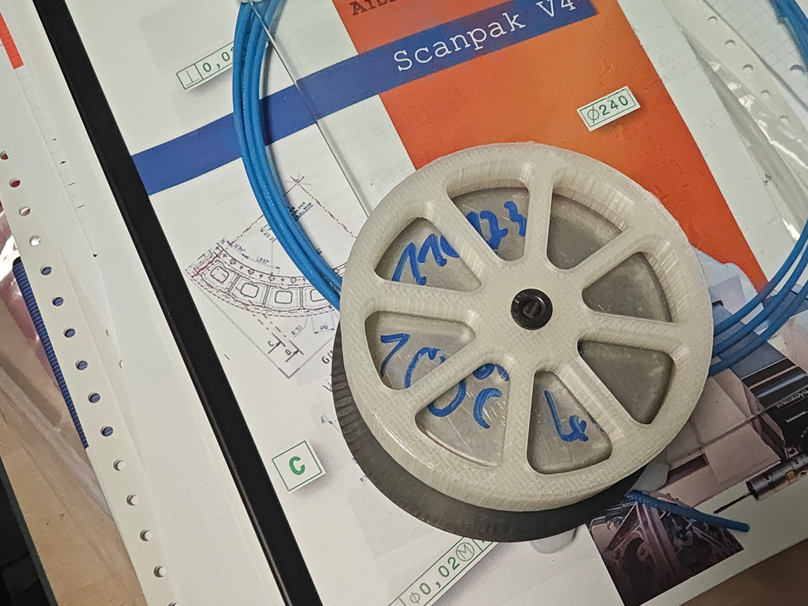
\includegraphics[width=\textwidth]{FiguresALL/Methodologie/méthodePerçage.png}
        \caption{Mise en place de l'emprunt sur un godet avant le perçage au centre}
        \label{fig:MethodePerçage}
    \end{minipage}
    \hfill
    \begin{minipage}[t]{0.45\textwidth}
        \centering
        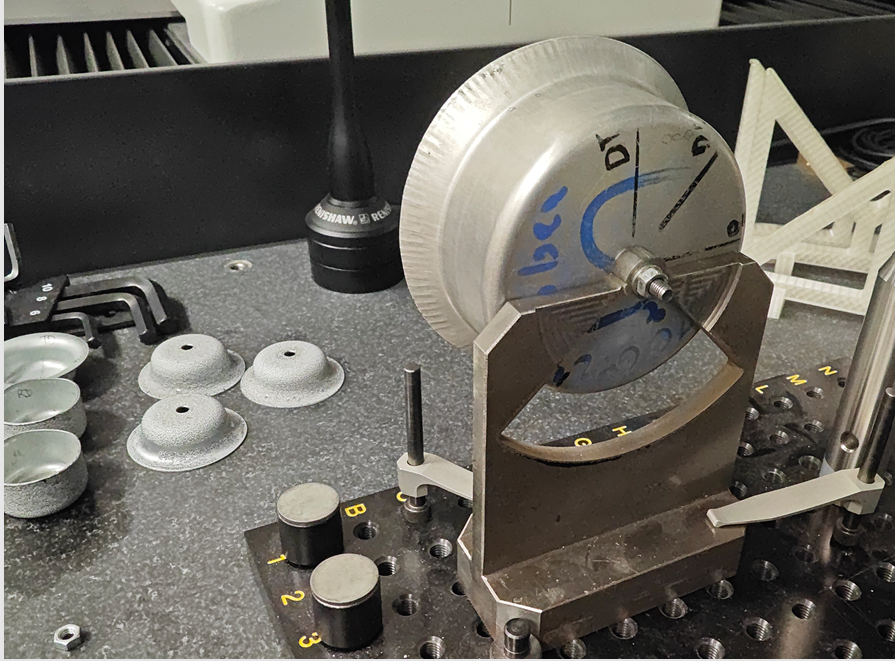
\includegraphics[width=\textwidth]{FiguresALL/Methodologie/fixationGodetOutils.png}
        \caption{Godet issu de l'étape2 d'emboutissage fixé sur le support }
        \label{fig:fixationGodet}
    \end{minipage}
\end{figure}
%fin Figure

Une fois que le godet est bien fixé sur son support selon la figure~\ref{fig:fixationGodet}, on le met en position sur la MMT grâce à une table taraudée sur laquelle on fixe des embouts pour éviter que le support de métrologie ne se déplace suivant le plan. Par ailleurs, la fixation hors plan est assurée avec deux butées, d'une part et d'autre du support, pour garantir une parfaite mise en position de notre pièce. Cela est illustré pour par la figure~\ref{fig:MisePosition}.

%Bloc figure modèle avec flèche
\begin{figure}[H]
    \centering
    \begin{tikzpicture}
        \node[anchor=south west, inner sep=0] (image) at (0,0)
            {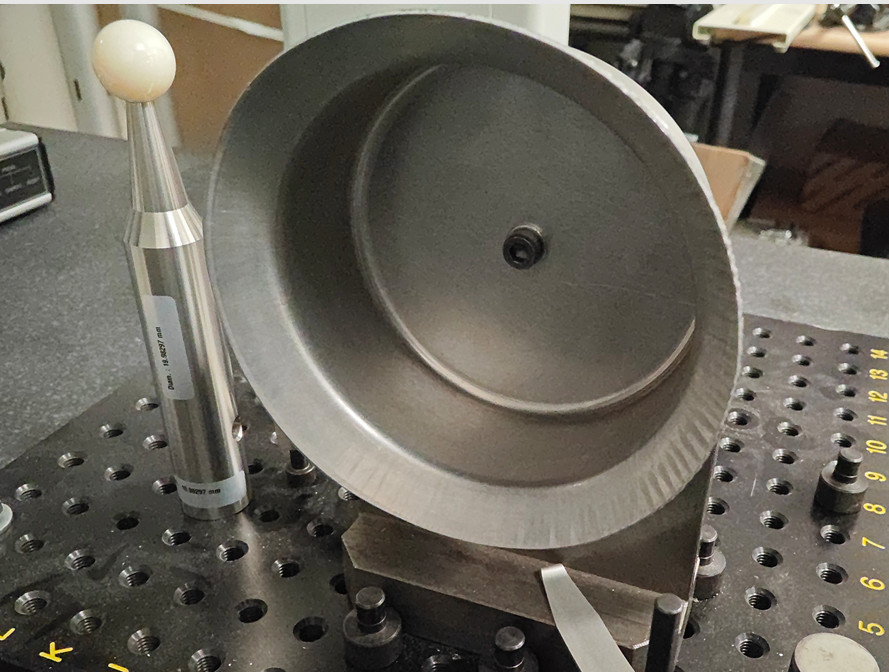
\includegraphics[width=0.4\textwidth]{FiguresALL/Methodologie/Mise en positionGodets.png}};

        \begin{scope}[x={(image.south east)}, y={(image.north west)}]

            \draw[->, thick, red]
                (0.1, 0.6) -- (0.42, 0.1);
            \node[red, font=\small\bfseries] at (0.14, 0.63)
                {Embouts};

            \draw[->, thick, blue]
                (0.8, 0.8) -- (0.63, 0.1);
            \node[white, font=\small\bfseries] at (0.85, 0.85)
                {Butée};
        \end{scope}
    \end{tikzpicture}
    \caption{Mise en position du support du godet sur la MMT}
    \label{fig:MisePosition}
\end{figure}

%sous titre pour expliquer comment on lance notre logiciel maintenant
%\subsubsection{Programme de mesure des profils}


%La MMT est commandée à travers un logiciel MCOSMOS qui fonctionne sur un ordinateur en liaison avec la machine. Une fois que toute la première étape, qui est la mise en position du godet sur la plaque de la machine est effectuée, un référentiel est défini, utilisé pour palper les nuages des points. Le plan ($\vec{y}$,  $\vec{z}$) est établi grâce au contact du palpeur sur trois points quelconques de la partie du support du godet illustré par la figure~\ref{fig:ref_plan}. Pour avoir l'origine du référentiel, quatre points sur l'extrémité du côté intérieur du godet sera mesuré ~\ref{fig:ref_origine}. La MMT utilisera ces 4 mesures pour déduire le centre de révolution du godet. Deux points alignés sont enfin palpés, encore sur le support de la pièce d'après la figure~\ref{fig:ref_axe} pour définir le sens de l'axe $\vec{y}$. Le référentiel établi est enregistré dans notre programme puis appelé une fois dans le programme à chaque lancement d'une expérience de mesure.   



%Bloc figure modèle
% \begin{figure}[H]
%     \centering

%     % -----------------------------------------------
%     % Sous-figure (a) : 3 points pour le plan (y,z)
%     % -----------------------------------------------
%     \begin{subfigure}[t]{0.30\textwidth}
%         \centering
%         \begin{tikzpicture}
%             \node[anchor=south west, inner sep=0] (image) at (0,0)
%                 {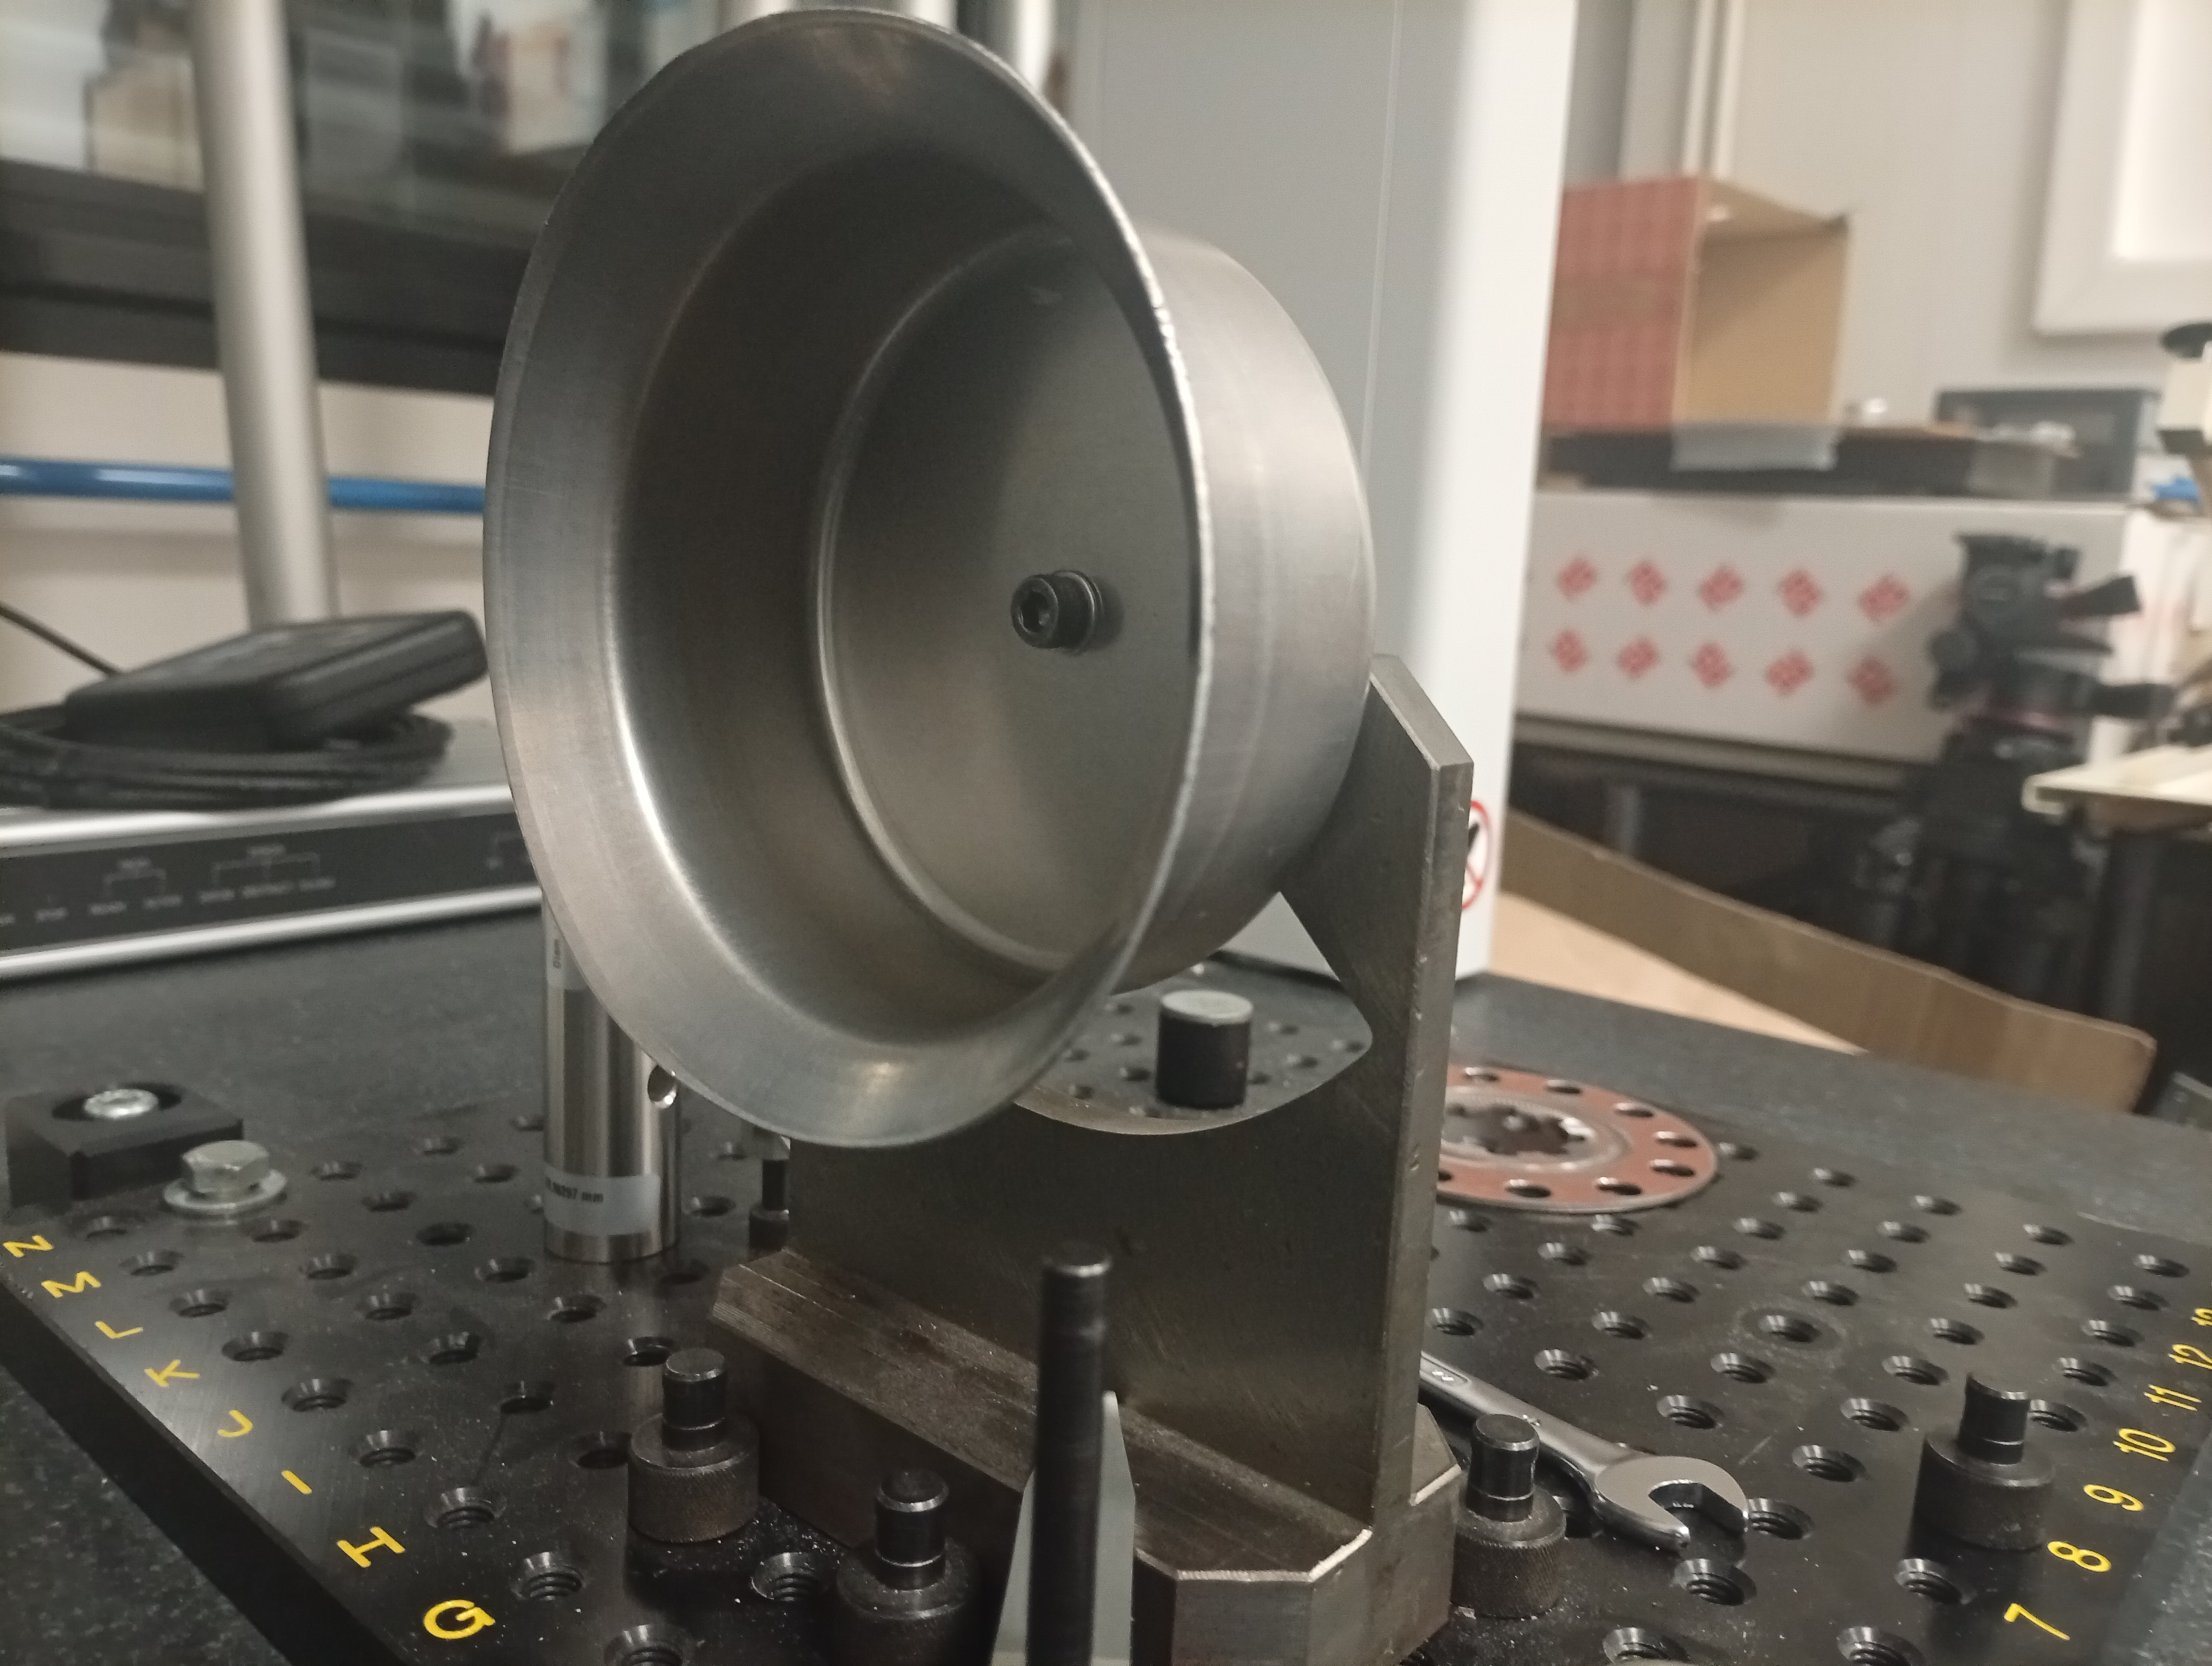
\includegraphics[width=\textwidth]{FiguresALL/Methodologie/référent.jpg}};
%             \begin{scope}[x={(image.south east)}, y={(image.north west)}]

%                 % Point 1
%                 \fill[red] (0.4, 0.27) circle (2pt);
%                 %\draw[red, thick] (0.25, 0.55) circle (7pt);
%                 \node[red, font=\bfseries\scriptsize] at (0.33, 0.27) {$P_1$};

%                 % Point 2
%                 \fill[red] (0.48, 0.3) circle (2pt);
%                 %\draw[red, thick] (0.50, 0.60) circle (7pt);
%                 \node[red, font=\bfseries\scriptsize] at (0.48, 0.36) {$P_2$};

%                 % Point 3
%                 \fill[red] (0.6, 0.2) circle (2pt);
%                 %\draw[red, thick] (0.75, 0.50) circle (7pt);
%                 \node[red, font=\bfseries\scriptsize] at (0.63, 0.22) {$P_3$};
%             \end{scope}
%         \end{tikzpicture}
%         \caption{3 points à mesurer pour le plan $(\vec{y},\vec{z})$}
%         \label{fig:ref_plan}
%     \end{subfigure}
%     \hfill
    % -----------------------------------------------
    % Sous-figure (b) : 4 points pour l'origine
    % -----------------------------------------------
%     \begin{subfigure}[t]{0.30\textwidth}
%         \centering
%         \begin{tikzpicture}
%             \node[anchor=south west, inner sep=0] (image) at (0,0)
%                 {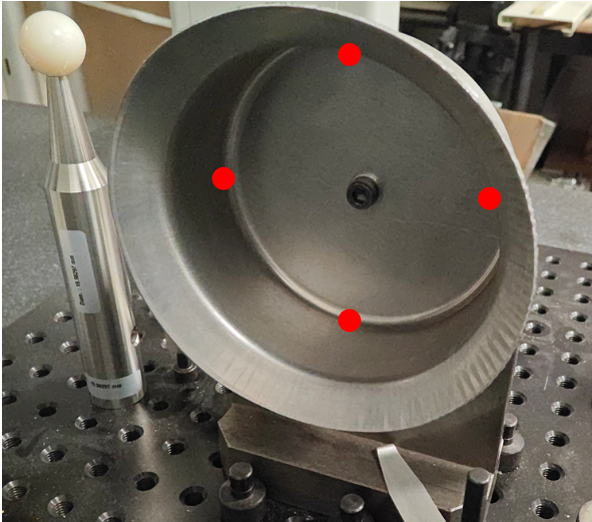
\includegraphics[width=0.85\textwidth]{FiguresALL/Methodologie/référentiel_origine.png}};
%             \begin{scope}[x={(image.south east)}, y={(image.north west)}]

%             \end{scope}
%         \end{tikzpicture}
%         \caption{4 points pour l'origine O}
%         \label{fig:ref_origine}
%     \end{subfigure}
%     \hfill
%     % -----------------------------------------------
%     % Sous-figure (c) : 2 points pour l'axe y
%     % -----------------------------------------------
%     \begin{subfigure}[t]{0.30\textwidth}
%         \centering
%         \begin{tikzpicture}
%             \node[anchor=south west, inner sep=0] (image) at (0,0)
%                 {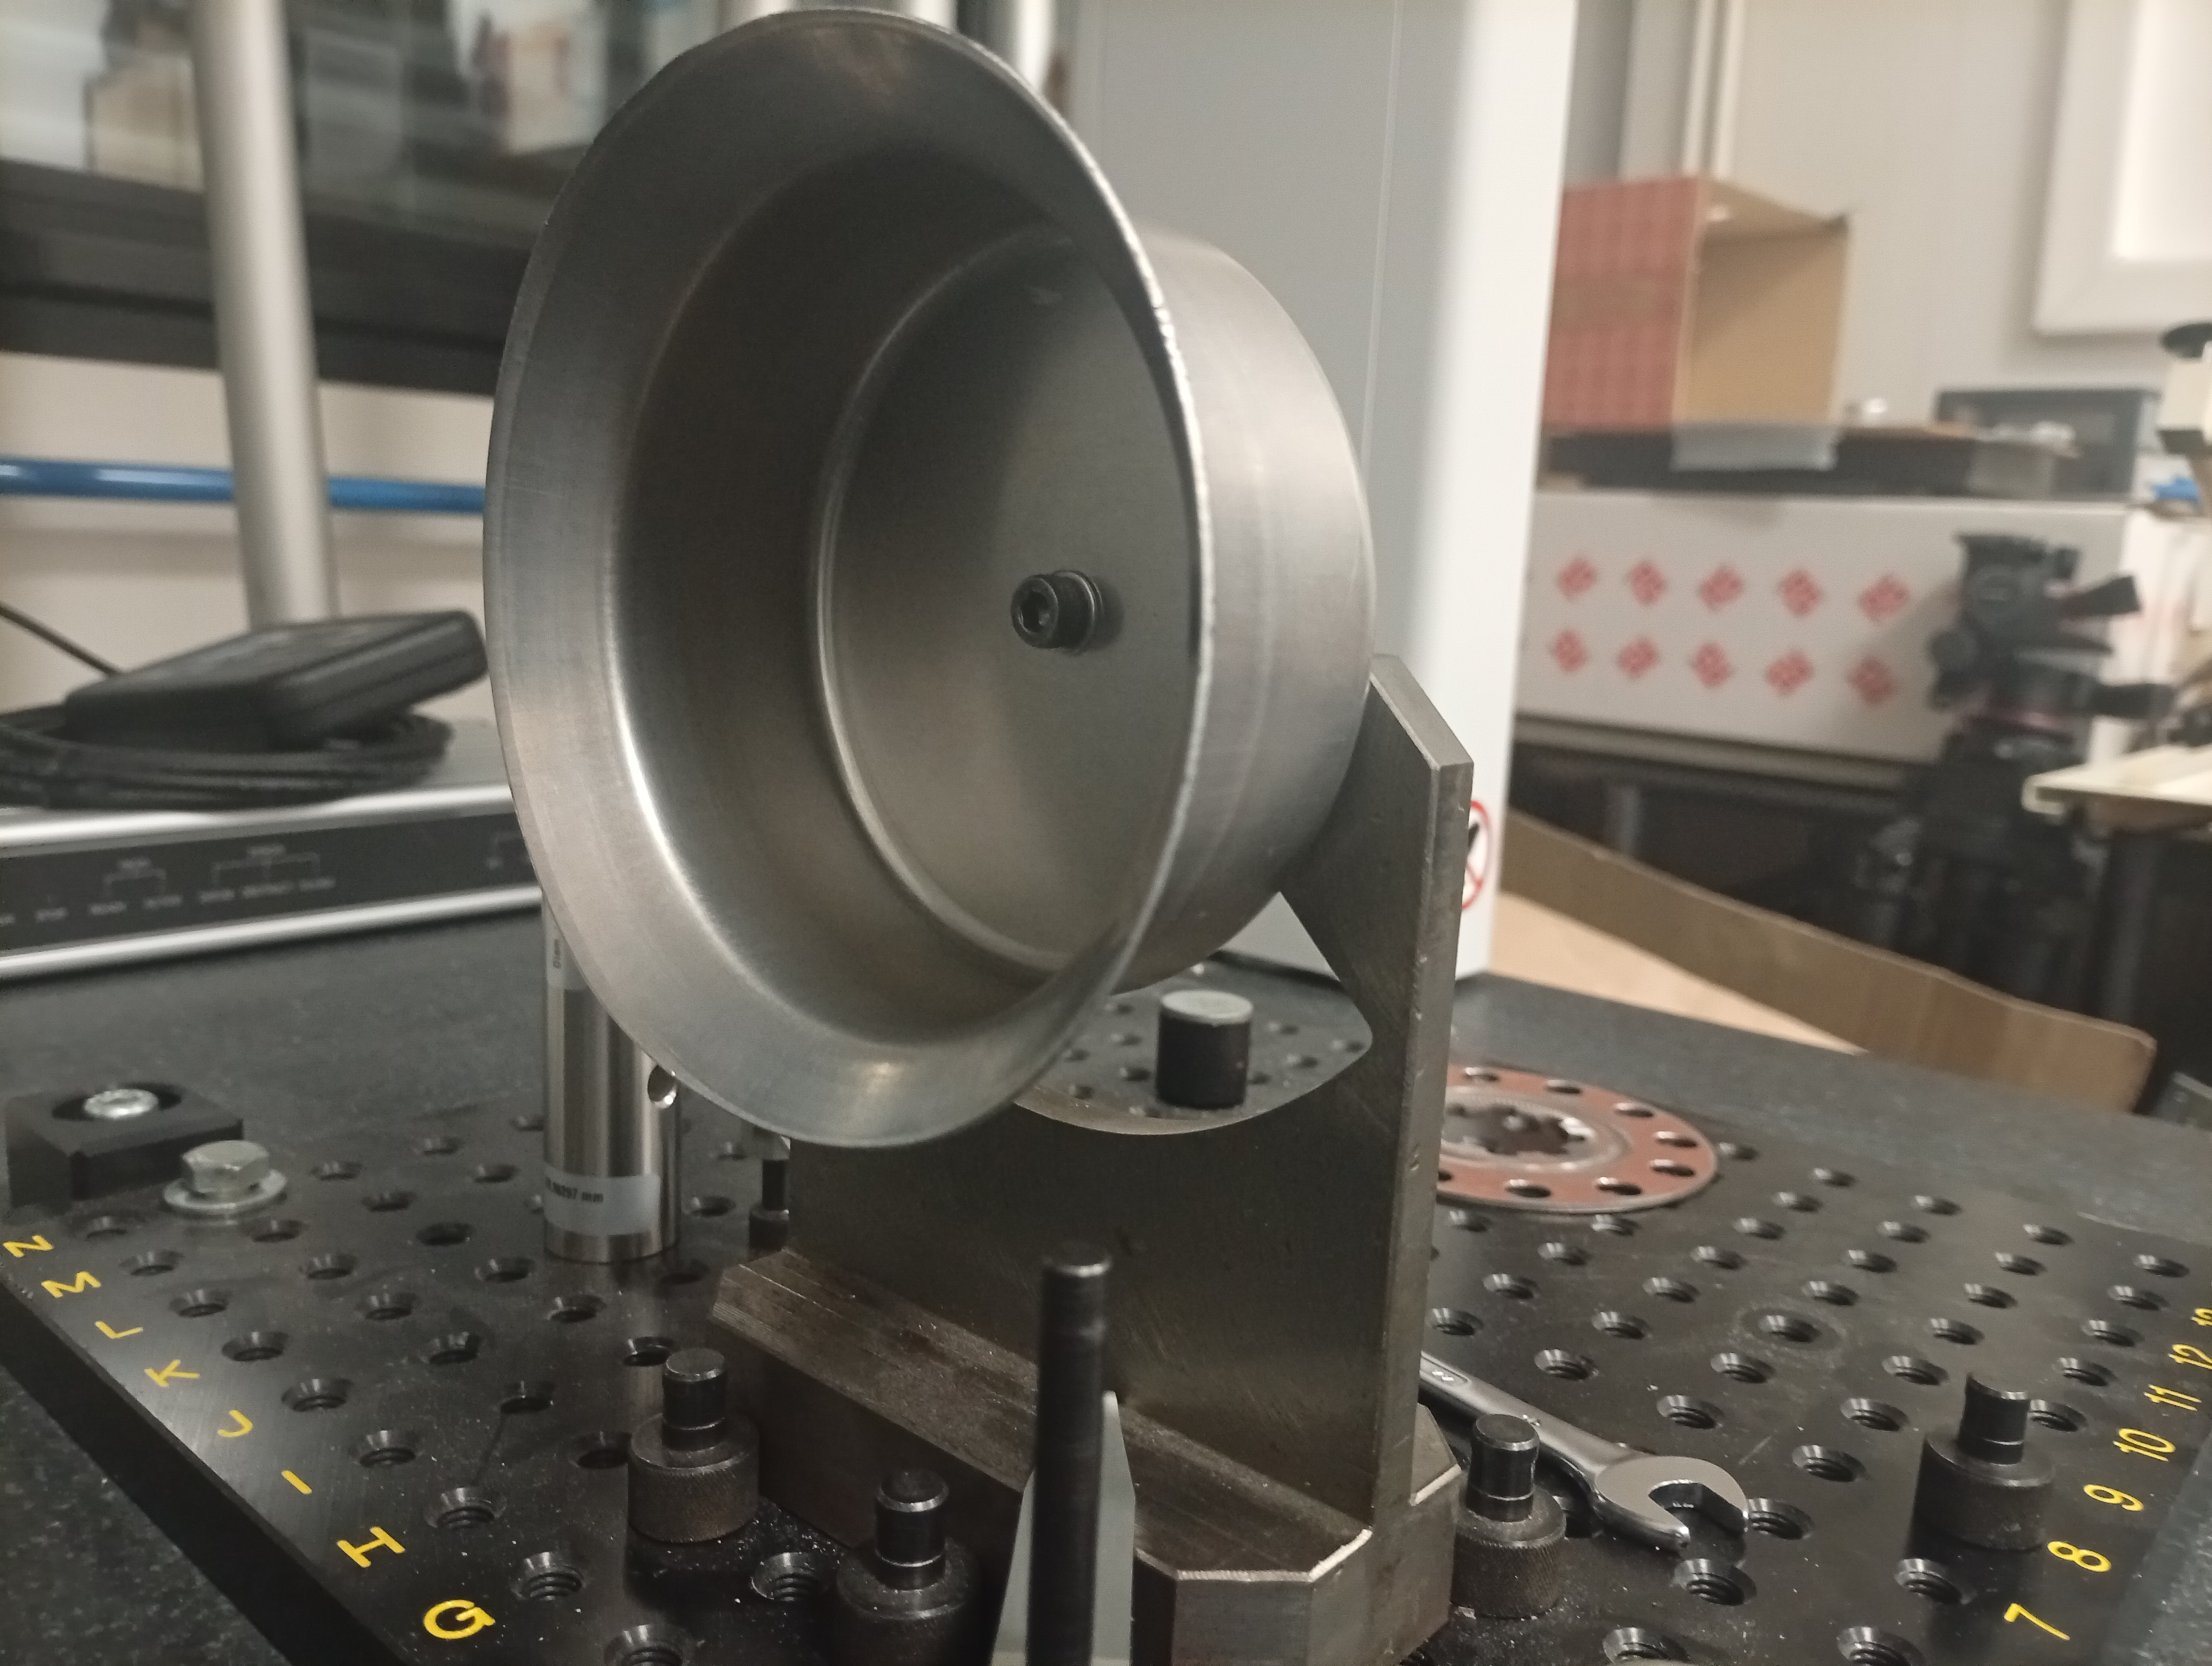
\includegraphics[width=\textwidth]{FiguresALL/Methodologie/référent.jpg}};
%             \begin{scope}[x={(image.south east)}, y={(image.north west)}]

%                 % 2 points alignés
%                 \fill[darkgreen] (0.62, 0.10) circle (2pt);
%                 %\draw[darkgreen, thick] (0.25, 0.50) circle (7pt);
%                 \node[white, font=\bfseries\scriptsize] at (0.68, 0.10) {$A$};

%                 \fill[darkgreen] (0.65, 0.50) circle (2pt);
%                 %\draw[darkgreen, thick] (0.75, 0.50) circle (7pt);
%                 \node[white, font=\bfseries\scriptsize] at (0.7, 0.58) {$B$};

%                 % Flèche axe y entre les deux points
%                 \draw[->, very thick, blue]
%                     (0.62, 0.10) -- (0.65, 0.50);
%                 \node[white, font=\scriptsize\bfseries] at (0.7, 0.45) {$\vec{y}$};
%             \end{scope}
%         \end{tikzpicture}
%         \caption{2 points pour l'axe $\vec{y}$}
%         \label{fig:ref_axe}
%     \end{subfigure}

%     \caption{Définition du référentiel de mesure : (a) plan $(\vec{y},\vec{z})$,
%              (b) origine du référentiel, (c) orientation de l'axe $\vec{y}$}
%     \label{fig:referentiel_complet}

% \end{figure}


%Figure du référentiel


%archive de texte original non reformulé
%La MMT est commandée à travers un logiciel MCOSMOS qui marche sur un ordinateur en liaison avec la machine. Une fois que toute la première étape, qui est la mise en position du godet sur la plaque de la machine est effectuée, un référentiel est défini, utilisé pour palper les nuages des points. Pour ce faire, le plan ($\vec{y}$,  $\vec{z}$) est établi grâce au contact du palpeur sur trois points quelconques de la partie du support du godet illustré par la figure (suivante). Pour avoir l'origine du référentiel, quatre points sur l'extrémité du côté intérieur du godet sera mesuré (Figure). La MMT utilisera ces 4 mesures pour déduire le centre de révolution du godet. Deux points alignés sont enfin palpés, encore sur le support de la pièce d'après la (Figure) pour définir le sens de l'axe $\vec{y}$. Le référentiel montré sur la (figure) établi est enregistré dans notre programme puis appelé à chaque lancement d'une expérience de mesure.
%end

 La  MMT est pilotée à l’aide du logiciel MCOSMOS, installé sur un ordinateur en communication directe avec la machine. Après la mise en position du godet sur la plaque de mesure, un référentiel est défini afin d’assurer la cohérence des acquisitions réalisées sur la pièce. 
 Le logiciel MCOSMOS fonctionne à partir de blocs de programme prédéfinis permettant de piloter séquentiellement les différentes opérations de mesure : déplacement du palpeur, scan de profil et export des données. Dans le cadre de cette étude, le programme de mesure développé par S. Royne \cite{royne_etude_2025} et J. Coër \cite{coer_mise_nodate} a été adapté pour l’acquisition automatisée des profils internes et externes du godet.
%Début Image
\begin{figure}[H]
    \centering
    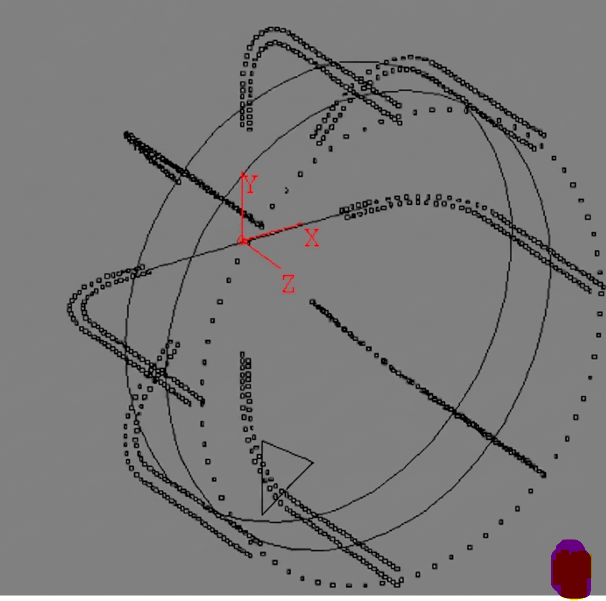
\includegraphics[width=0.6\textwidth]{FiguresALL/Methodologie/representationDiscrete_godets.png}
    \caption{Représentation en 3D de l'ensemble des profils mesurés expérimentalement}
    \label{fig:DiscretRepresente}
\end{figure}
%fin Image
 Le palpeur mesure des points discrets le long de chaque profil du godet tous les (45°), en commençant à (0°) par rapport à la Direction de Laminage (DL), afin de couvrir l’ensemble du contour de la pièce. Les coordonnées tridimensionnelles $(\vec{x},\vec{y},\vec{z})$ des points mesurés sont automatiquement enregistrées dans un fichier texte. La figure~\ref{fig:DiscretRepresente} présente l’ensemble des points acquis reconstruisant la géométrie globale du godet.

 
%La figure~\ref{fig:ExProgramme} montre une partie du programme utilisé pour la mesure de profil. 


%Bloc figure modèle
%\begin{figure}[H]                          % [H] = figure exactement ICI dans le texte
    %\centering                             % centrage de l'image
    %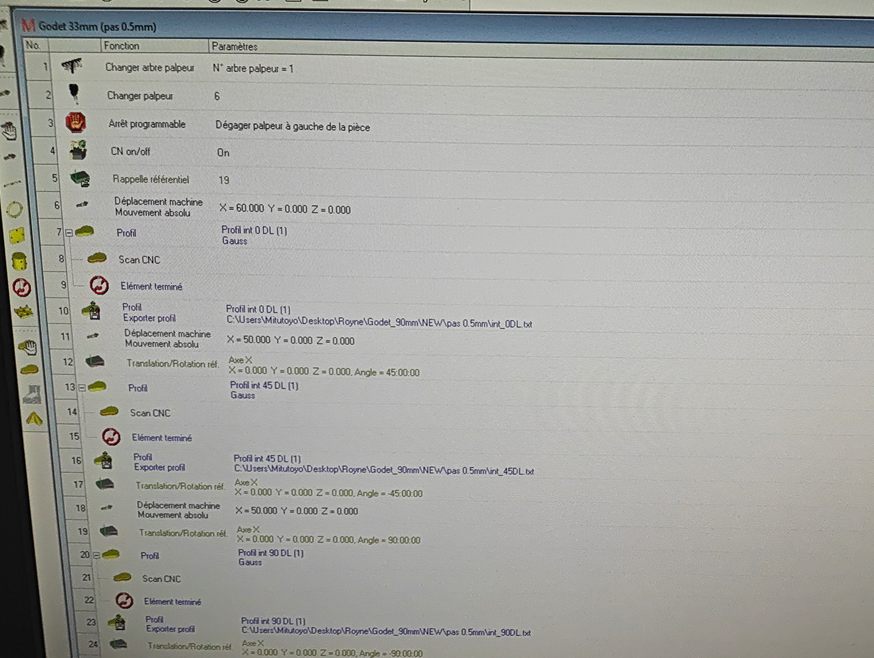
\includegraphics[width=0.5\textwidth]{FiguresALL/Methodologie/ProgrammeMachine.png}  % chemin + taille
    %\caption{Exemple de programme sous MCOSMOS pour l’acquisition de profils}   % légende affichée sous l'image
   % \label{fig:ExProgramme}                  % étiquette pour rappeler la figure
%\end{figure}
%fin figure




%Méthodologie pour le calcul d'épaisseur 




\subsection{Calcul de l'épaisseur et distance curviligne}
Expérimentalement, les points, représentants les profils du godet de l'étape 1
(figure~\ref{fig:Step1Emboutissage}) et de l'étape 2 (figure~\ref{fig:Step2Emboutissage})
ont été recueillis suivant les directions de son contour avec un incrément de 45° selon la figure~\ref{fig:DiscretRepresente}. Chaque direction de profil est représenté en 2D, selon la figure~\ref{fig:DiscretRepresente2D} pour faciliter son exploitation pour le calcul de l'épaisseur.  
%Début Image
\begin{figure}[H]
    \centering
    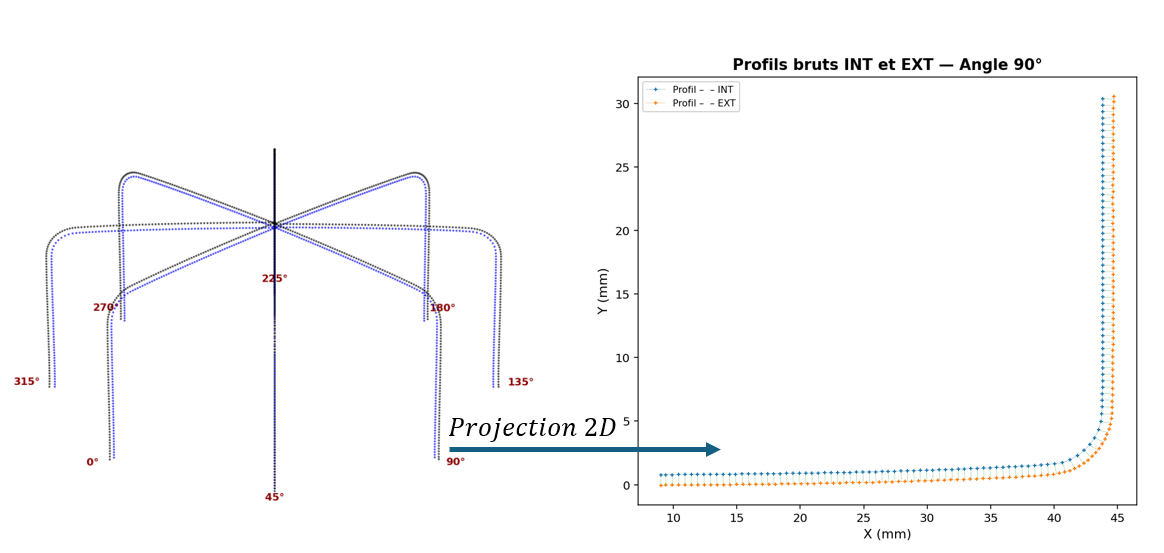
\includegraphics[width=0.6\textwidth]{FiguresALL/Methodologie/représentation2D_3D.png}
    \caption{Projection de deux profils représentant une direction, cas de la direction 90° par rapport à la DL}
    \label{fig:DiscretRepresente2D}
\end{figure}
%fin Image

L'épaisseur locale est définie, d'après~\cite{xin_intrinsic_2016}, comme la distance entre un point d'un profil et son intersection avec le profil opposé, mesurée le long de la normale locale.

La méthode pour avoir l'épaisseur locale, à travers deux profils intérieurs et extérieurs du godet, se décompose en quatre étapes successives, appliquées à chaque point du profil extérieur.

%──────────────────────────────────────
\subsubsection{Calcul de la normale locale}
%\paragraph{Étape\,1 — Calcul de la normale locale}
%\mbox{}\\
%L’épaisseur locale est mesurée suivant la normale à l’une des surfaces, interne ou externe, du godet. Il faut donc, pour chaque point mesuré, déterminer la direction normale au profil en ce point. 
Dans un premier temps, une normale locale est déterminée en chaque point du profil extérieur. Pour ce faire, le vecteur tangent unitaire \(\vec{e}_1\) entre deux points consécutifs du profil choisi s'écrit :
\[
\vec{e}_1
=
\frac{
\overrightarrow{P_i^{ext}P_{i+1}^{ext}}
}{
\left\|
\overrightarrow{P_i^{ext}P_{i+1}^{ext}}
\right\|
}
\tag{2}
\]
Le profil étant plan, la normale dans ce plan est obtenue par produit vectoriel
avec le vecteur hors-plan \(\vec{e}_3 = (0,\,0,\,1)\) :
\[
    \vec{n} = \vec{e}_1 \wedge \vec{e}_3
    \quad\Longrightarrow\quad
    \vec{n} = \begin{pmatrix} e_{1y} \\ -e_{1x} \end{pmatrix}
    \tag{3}
\]
Cette opération est répétée pour chaque point du profil, fournissant ainsi
une normale locale à la géométrie réelle (mur, rayon, fond).

\begin{figure}[H]
    \centering
    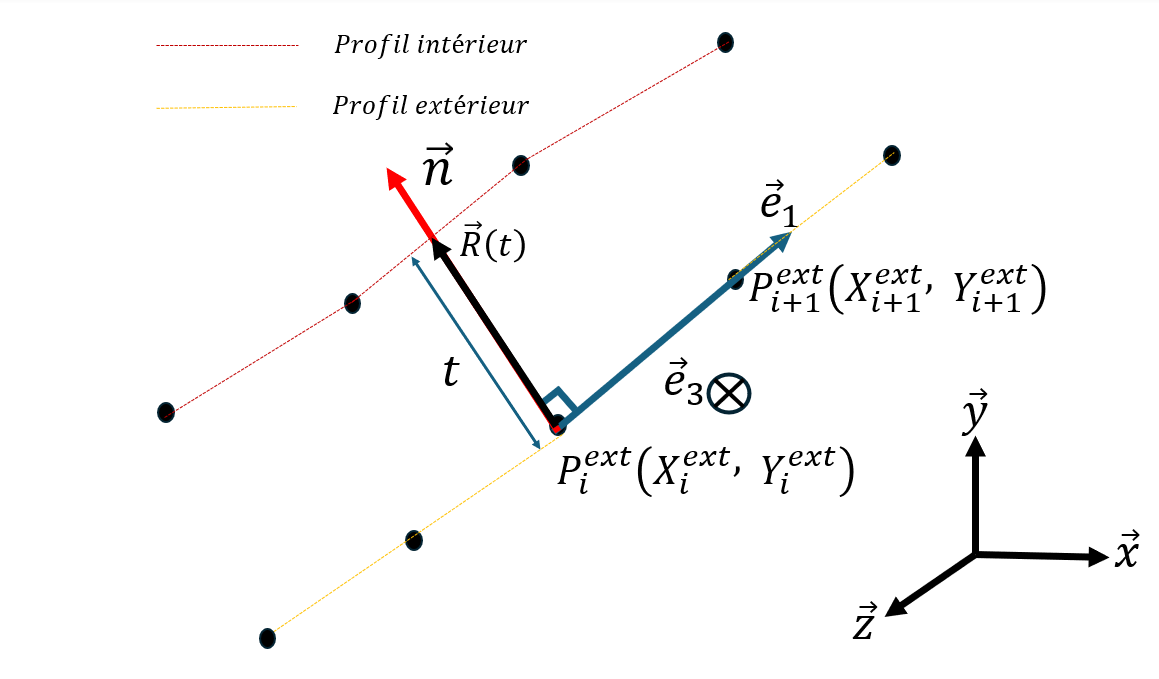
\includegraphics[width=0.6\textwidth]{FiguresALL/Methodologie/Calcul_Normale_Version_Finale.png}
    \caption{Calcul du vecteur Normale $\vec{n}$ et sa projection $\vec{R}(t)$  depuis un point du profil extérieur}
    \label{fig:normale}
\end{figure}

%──────────────────────────────────────
\subsubsection{Recherche de l'intervalle d'intersection par rapport au profil opposé du point extérieur projeté}
%\paragraph{Étape\,2 --- Lancement du rayon et recherche de l'intervalle}
%\mbox{}\\
%New Version

Une fois la normale unitaire \(\vec n = (N_x,N_y)\) déterminée au point
extérieur projeté \(P^{ext}=(P_x^{ext},P_y^{ext})\), un rayon \(R(t)=(X(t),Y(t))\) est projeté depuis ce point
dans la direction de \(\vec n\), comme illustré à la
figure~\ref{fig:normale}.

On obtient alors la paramétrisation :
\begin{equation}
R(t)=
\begin{pmatrix}
X(t) \\
Y(t)
\end{pmatrix}
=
\begin{pmatrix}
P_x^{ext} \\
P_y^{ext}
\end{pmatrix}
+
t
\begin{pmatrix}
N_x \\
N_y
\end{pmatrix},
\qquad t \ge 0
\tag{4}
\end{equation}

Le vecteur \(\vec n\) étant normalisé, le paramètre \(t\) correspond
directement à l'épaisseur que l'on souhaite avoir, exprimée en mm.

L'objectif est alors de déterminer la valeur \(t\) pour laquelle le
rayon intersecte le profil intérieur.




%ARCHIVE ANCIENNE VERSION
% Une fois la direction de la normale connue, on projette un rayon depuis le point sur le profil extérieur choisi, noté : 
% \(\vec{P}_{ext} = (P_x,\,P_y)\) dans la direction \(\vec{n}\),
% et paramétré par la distance \(t\) selon la figure~\ref{fig:normale} :
% \begin{equation}
%     \vec{R}(t) = \vec{P}_{ext} + t\cdot\vec{n}
%     = \begin{cases}
%         X_{ray}(t) = P_x + t\,N_x \\
%         Y_{ray}(t) = P_y + t\,N_y
%     \end{cases}
%     \tag{4}
% \end{equation}
% Puisque \(\vec{n}\) est unitaire, le paramètre \(t\) est directement
% l'épaisseur locale en mm. Il reste à trouver la valeur de \(t\) pour laquelle
% cette projection touche le profil intérieur.

Le profil intérieur étant discret, l’intersection ne peut pas être résolue directement.
Il est donc nécessaire d’identifier au préalable le segment du profil intérieur
intersecté par la projection normale.

L’approche proposée consiste à déterminer l’intervalle défini par deux points consécutifs
du profil intérieur sur lequel le rayon \(R(t)\) intersecte ce dernier.

Pour ce faire, on calcule la distance euclidienne entre
\({P}^{ext}\) et chaque point intérieur \(P_j^{int}\) :
\[
    d_j^2 = \bigl(X_j^{int} - P_x^{ext}\bigr)^2 + \bigl(Y_j^{int} - P_y^{ext}\bigr)^2
    \tag{5}
\]
\begin{figure}[H]
\centering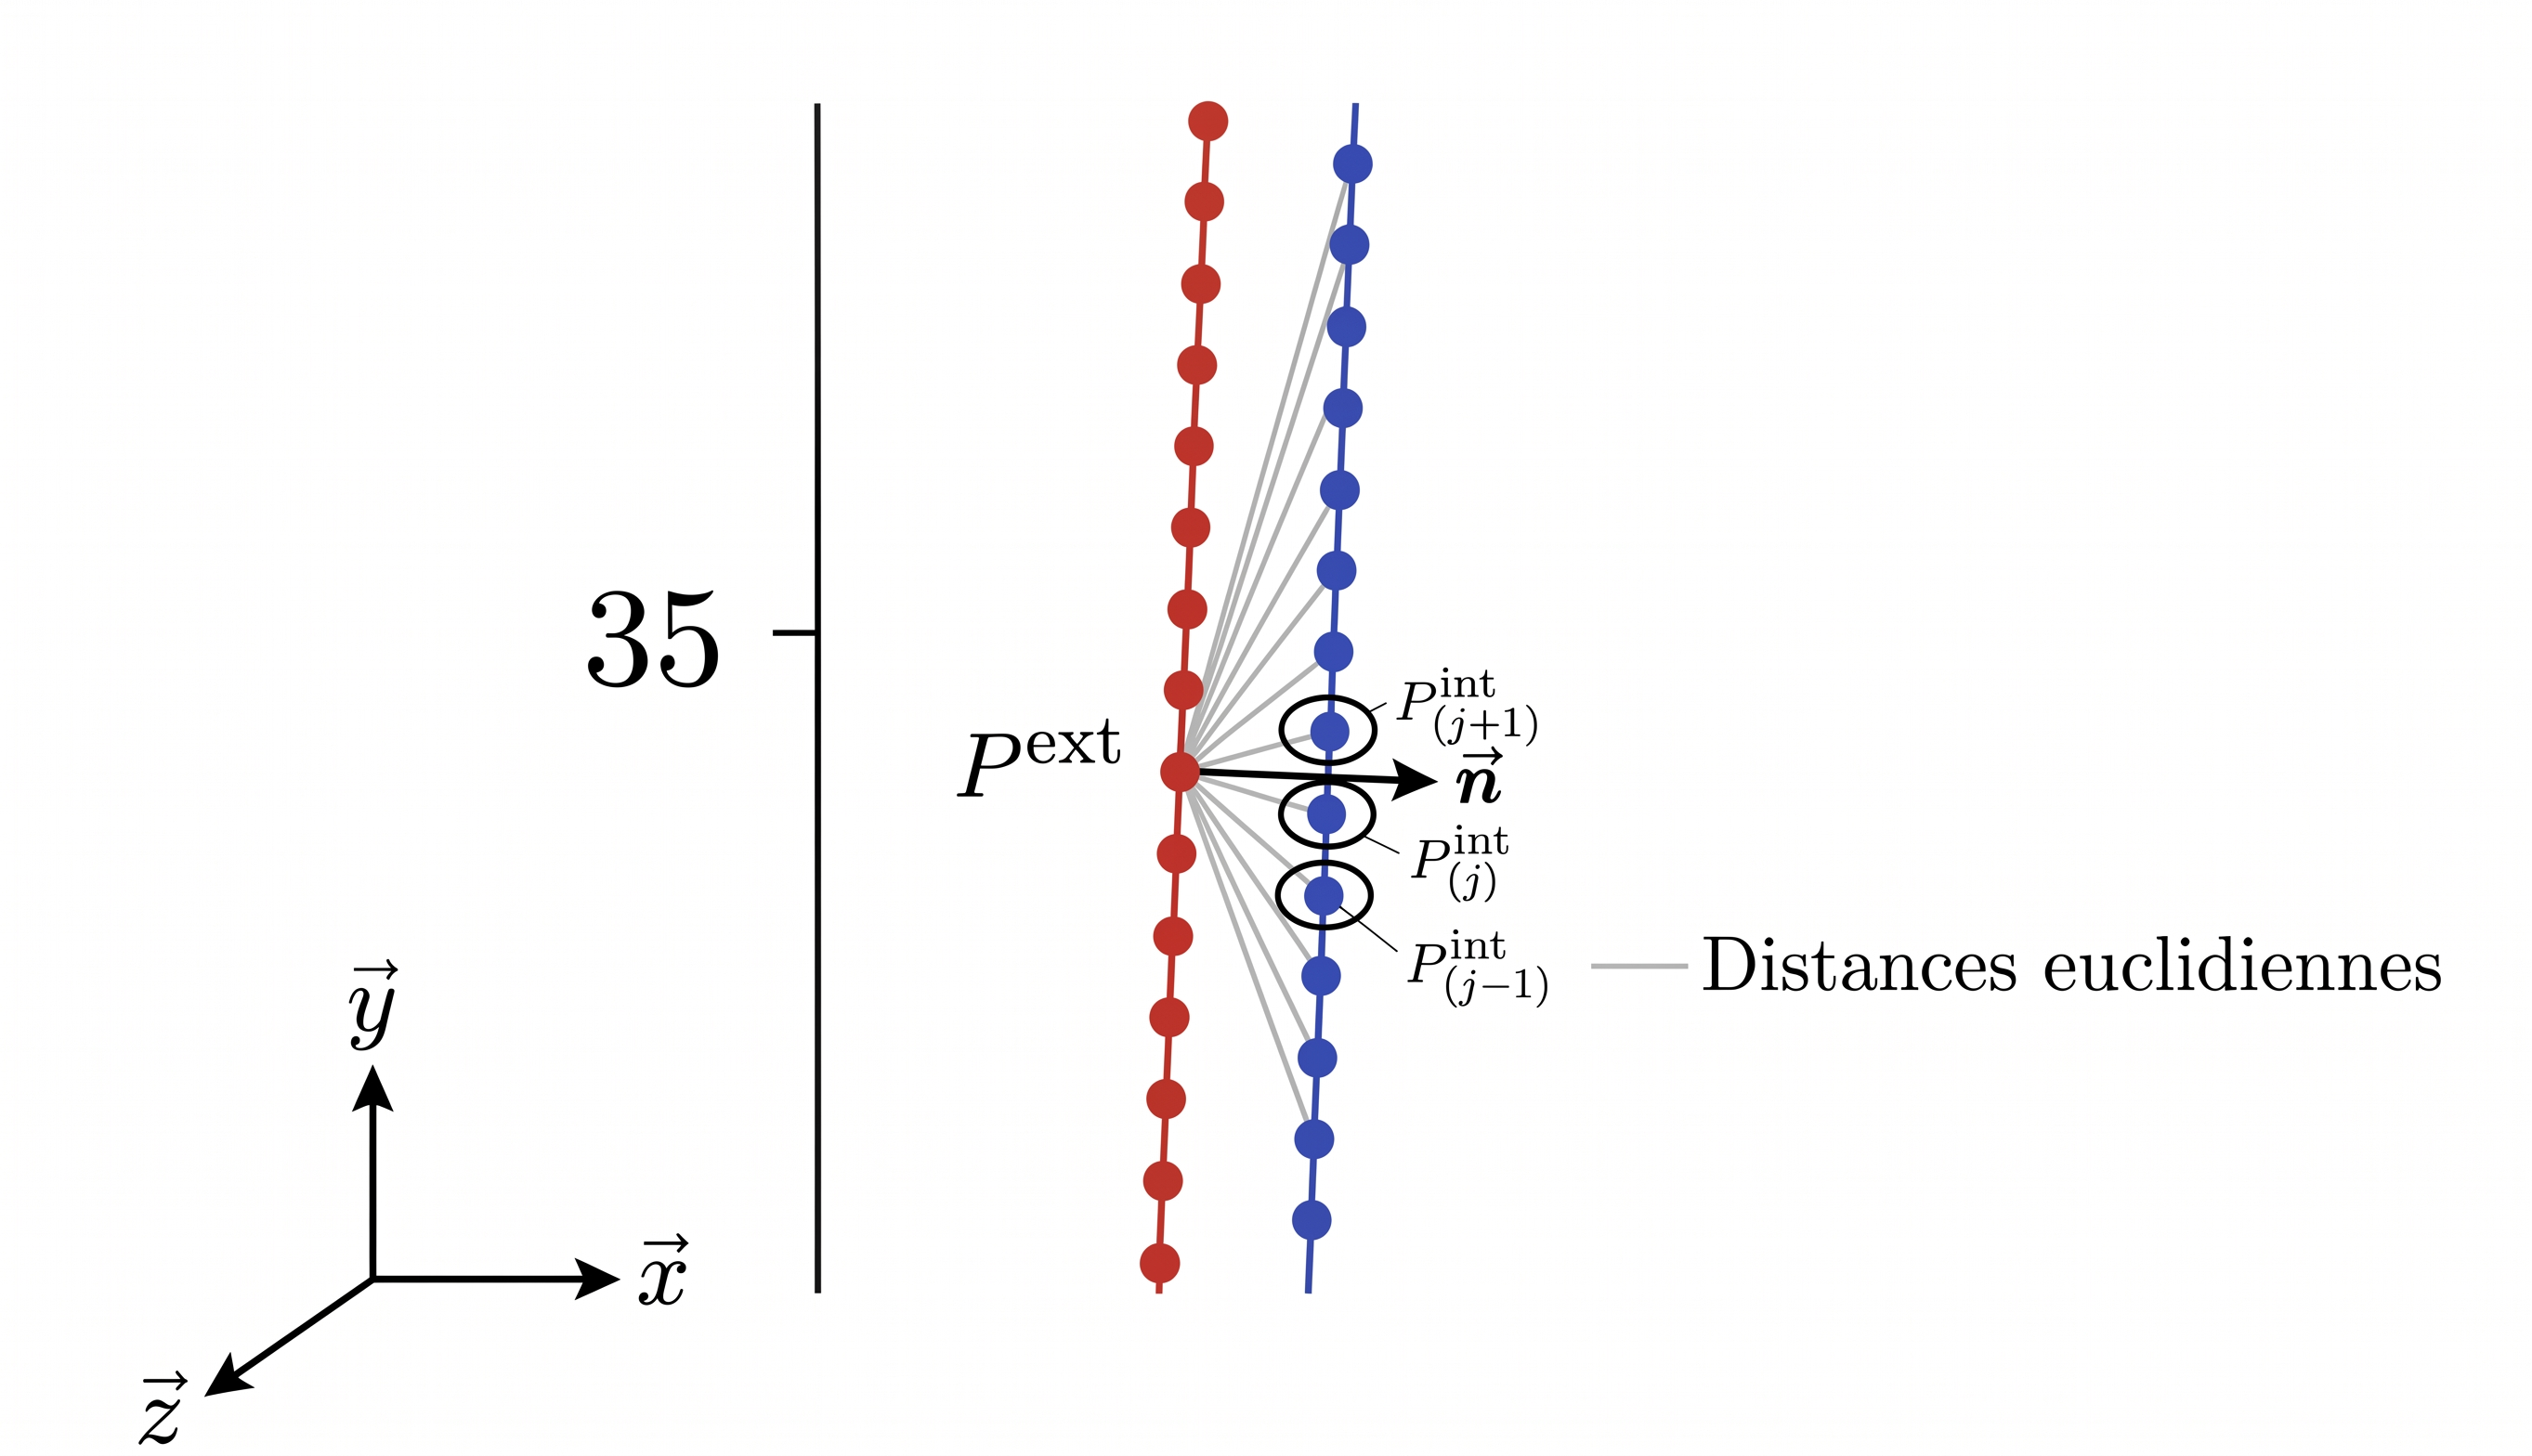
\includegraphics[width=0.6\textwidth]{FiguresALL/Methodologie/euclidienne_Version_Finale_Vrai.png}
    \caption{Distances euclidiennes entre le point extérieur projeté \(P^{ext}\) et les points intérieurs candidats
    \(P_{j-1}^{int}\), \(P_j^{int}\) et \(P_{j+1}^{int}\).}
    \label{fig:distances}
\end{figure}
Les 3 points les plus proches \(P_{j-1}^{int},\; P_j^{int},\; P_{j+1}^{int}\)
de la figure~\ref{fig:distances} sont retenus comme candidats à l'intersection.

Le segment intersecté par le rayon est identifié à l’aide d’un critère de colinéarité.
Pour chaque point intérieur candidat \(P_j^{int}\), le vecteur reliant le point
extérieur projeté \(P^{ext}\) à ce point est défini par
\(\vec u_j = P_j^{int} - P^{ext}\).

Le rayon \(R(t)\) intersecte alors le segment
\([P_j^{int},\,P_{j+1}^{int}]\) si seulement si le déterminant entre
\(\vec u_j\) et la normale \(\vec n\) s’annule :

\[
f_j
=
\det(\vec u_j,\vec n)
=
\left(X_{j}^{int}-P_x^{ext}\right)N_y
-
\left(Y_{j}^{int}-P_y^{ext}\right)N_x
\tag{6}
\]


Un changement de signe entre deux valeurs consécutives indique que le rayon
traverse ce segment, d'après le théorème des valeurs intermédiaires :
\[
    f_{j-1}\cdot f_j < 0
    \quad\Longrightarrow\quad
    \text{intersection dans }
    \bigl[P(j-1),\;P(j)\bigr]
\]

%──────────────────────────────────────

\subsubsection{Calcul de l'épaisseur entre le profil intérieur et extérieur}
%\paragraph{Étape\,3 — Résolution par égalité vectorielle}
%\mbox{}\\
L'intervalle $[P(j),\,P(j+1)]$ étant identifié, le segment intérieur est
paramétré par $s \in [0,1]$ :
\[
    \overrightarrow{P_j P_{j+1}}(s) = P_j + s\cdot\bigl(P_{j+1} - P_j\bigr)
    \tag{7}
\]
Le point d'intersection est la solution de l'égalité vectorielle
$\vec{R}(t) = \overrightarrow{P_j P_{j+1}}(s)$,
qui se décompose en un système linéaire $2 \times 2$ :
\[
    \begin{cases}
        t\,N_x - s\,(X_{j+1}-X_j) = X_j - P_x \\[4pt]
        t\,N_y - s\,(Y_{j+1}-Y_j) = Y_j - P_y
    \end{cases}
    \tag{8}
\]
La résolution fournit simultanément :
\begin{itemize}
    \item $t^* \equiv e$ : \textbf{l'épaisseur locale} (en mm),
    distance réelle entre les deux profils suivant la normale ;
    \item $s^*$ : la position du point de contact sur le segment intérieur,
    permettant de localiser précisément le point d'impact.
\end{itemize}
Ces quatre étapes sont répétées pour chacun des points du profil extérieur,
reconstituant ainsi l'évolution complète de l'épaisseur le long du godet.

%──────────────────────────────────────
\subsubsection{Épaisseur en fonction de la distance curviligne}
%\paragraph{Étape\,4 --- Représentation sur la distance curviligne médiane}
%\mbox{}\\
Pour représenter l'épaisseur de façon physiquement significative et comparable
entre profils de géométries différentes, on utilise la \textbf{distance curviligne}
notée \(s_j\), calculée point par point par la formule de Pythagore discrète :
\[
    \Delta s_j = \sqrt{\bigl(X_{j+1} - X_j\bigr)^2 + \bigl(Y_{j+1} - Y_j\bigr)^2}
    \tag{9}
\]
\[
    s_j = \sum_{k=0}^{j-1} \Delta s_k
    \tag{10}
\]

\begin{figure}[H]
    \centering
    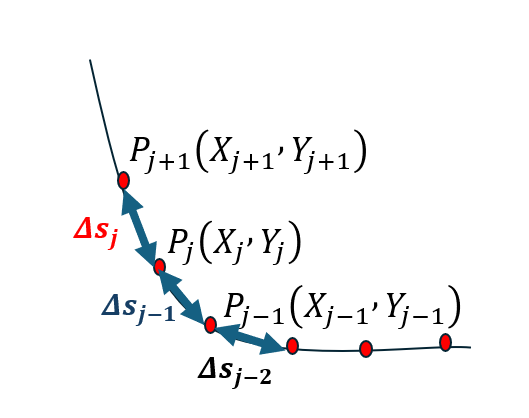
\includegraphics[width=0.6\textwidth]{FiguresALL/Methodologie/dista_curvv.png}
    \caption{Définition de la distance curviligne}
    \label{fig:curviligne}
\end{figure}

D'après les travaux de \cite{coer_mise_nodate}, cette distance curviligne
n'est pas calculée sur le profil extérieur ni sur le profil intérieur,
mais sur la \textbf{ligne médiane} --- définie comme la courbe passant
exactement à mi-épaisseur en chaque point :
\[
    P_j^{med} = P_j^{ext} + \frac{t^*}{2}\,\vec{n}_j
    \tag{11}
\]
\[
    s_j^{med} = \sum_{k=0}^{j-1}
    \sqrt{\bigl(X_{k+1}^{med} - X_k^{med}\bigr)^2
    + \bigl(Y_{k+1}^{med} - Y_k^{med}\bigr)^2}
    \tag{12}
\]

\begin{figure}[H]
    \centering
    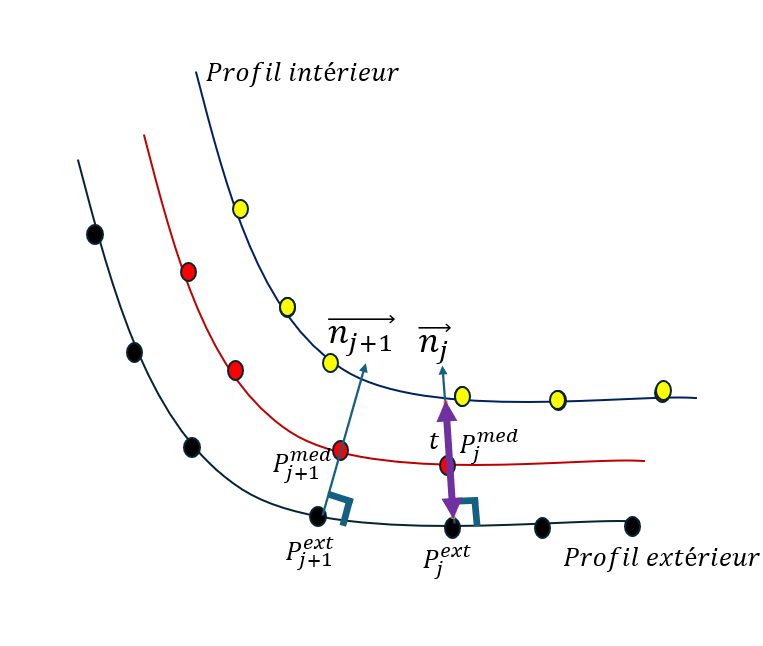
\includegraphics[width=0.6\textwidth]{FiguresALL/Methodologie/dist_mediane.png}
    \caption{La distance curviligne médiane $s_j^{med}$}
    \label{fig:mediane}
\end{figure}

Ce choix garantit une abscisse indépendante du profil de référence
et permet une comparaison directe entre les zones du godet
(fond, rayon, mur) ainsi qu'entre différents godets.

%Selon la défintion de l'épaisseur d'un profil par l'article(), qui est la distance de la projection normale d'un point sur un profil en intersection avec l'autre profil opposé. Pour avoir l'évolution de l'épaisseur tout le long d'un profil, il faut faire une opération de projection par rapport à sa normale et rechercher son intersection avec l'autre profil à chaque point du profil projeté.
%Ce qui nous a amené à faire ces opérations suivants pour chaque point du profil intérieur pour avoir l'épaisseur réelle du godet. 

%Recherche de la normale du point pour chaque profil : 
%Cette étape consiste d'abord à prendre chaque point du profil et à tracer une droite qui la relie avec le point du suivant conformément à la figure. On va appeler cette droite e1 de composant connu() qui est normale par rapport à l'axe eZ hors plan qu'on considère comme composants eZ(0,0,1). En faisant le produit vectorielle de ces deux axes e1 et eZ, les composantes de la normales de e1 sur le plan est retrouvé dont on va appelé n(vecteur).

%Lancer de la normale du point et recherhce de l'intervalle d'intersection. 
%Une fois que la normale est retrouvée, on va la lancée le long de l'autre Profil avec comme paramètre de distance t qui avec la formule de Rayon lancée : 
%Equation
%t est la distance du point de contact entre la normale projetée et le profil opposé. 
%C'est la recherche de ce point d'intersection entre la normale lancée et le profil opposé qui nous pose problème donc on doit faire d'abord une recherche de l'intervalle de contact. Pour se faire on calcule la distance entre le point projeté et tous les points du profil de l'extérieur et on retient les 3 distances qui sont les plus proches de ce point. Pour savoir, le vrai intervalle de l'intersection entre ces 2 distances , on avait utiliser le principe de la colinéarité des vecteur, entre le vecteur projeté R et les vecteurs entre les points les plus proches et le point projeté. (Ecrire l'équation) Qui nous enmène à dire que si les on est en intersection cette équation sera à 0. Et d'après, la méthode de l'encadrement de la solution 0, on peut dire que le point d'intersection se situe entre l'intervalle où il est changement de signe. 
%Une fois que l'intervalle est retrouvé, on vient faire à la fin une égalité vectorielle entre la projection lancée avec t comme distance et le vecteur entre les deux points succéssifs des deux intervalles. On obtient une équation du second degré avec deux inconnus qui sont t équivaut à l'épaisseur et (l'autre) distance d'intersection sur le vecteur de l'intervalle. Pour avoir l'épaisseur maintenant le long de tout le profil, il suffit de faire ces mêmes étapes pour l'ensemble des points intérieurs mesurés.


%Afin d'avoir une représentativité de la distribution de l'épaisseur le long du profil du godet. Selon les travaux de (Jeremy coer encore), on vient représenter l'épaisseur sur sa distance curviligne médiane. Avec, le point médiane est la moitié de l'épaisseur t et qui se définit comme la cumul de distance entre chaque point du milieu de l'épaisseur. (equation)
%Dans ce cadre on peut visualiser plus proprement l'évolution de l'épaisseur sur un profil.




%Le post-traitement de ces points nous permettrons de retrouver l'évolution de l'épaisseur tout au long d'un profil comme ce qu'a déjà réalisé \cite{coer_mise_nodate}. L'objectif est de recueillir l'épaisseur sur chaque partie du profil afin de regarder son évolution en fonction de la distance curviligne médiane des godets. L'épaisseur 
\subsection{Simulation Numérique de l'emboutissage en 2 étapes}

%Explication du modèle numérique sur simulation numérique
\subsubsection{Présentation du modèle éléments finis en 2D axisymétrique}

%Version Brute sans correction
%Du côté de la simulation numérique, le logiciel exploité était ABAQUS avec un modèle de calcul explcit. Dans un premier temps, le modèle de référence pris en compte était celui dans l'article de \cite{royne_etude_2025}.  
%Un modèle axisymétrique 2D est utilisé pour représenter les deux étapes d’emboutissage, afin de réduire le temps de calcul et de permettre une première validation de la simulation de l'emboutissage\cite{royne_etude_2025}. Dans cette phase initiale, le retour élastique ainsi que l’anisotropie du matériau ne sont pas pris en compte. Les deux étapes ont été simulés à travers deux étapes de calculs de type 'STATIC' sur le logiciel dont lequel l'étape 2 reprend directement l'état final du premier godet embouti. Le modèle de comportement élasto-plastique isotrope et isotherme de la loi de SWIFT a été repris selon \cite{royne_etude_2025}. De même, Le type et le nombre de maille utilisé dans\cite{royne_etude_2025} a été réutilisé après avoir fait une étude de convergence. Enfin,les conditions limites ainsi que les interactions, déjà détaillés dans \cite{royne_etude_2025} seront récapitulés par la figure(SUIVANTE).

Du côté de la simulation numérique, le logiciel exploité est ABAQUS 
avec une résolution de type \textit{Static}. Dans un premier temps, le modèle de 
référence retenu est celui développé par S.Royne \cite{royne_etude_2025}. 
Un modèle axisymétrique 2D est utilisé pour représenter les deux 
étapes d'emboutissage, afin de réduire le temps de calcul et de 
permettre une première validation numérique. 
Dans cette phase initiale, le retour élastique ainsi que l'anisotropie 
du matériau ne sont pas pris en compte. Les deux étapes sont simulées 
séquentiellement, l'étape 2 reprenant directement l'état déformé final 
du premier godet embouti. Le modèle de comportement élasto-plastique 
isotrope et isotherme de type Swift a été retenu conformément au travail de S.Royne 
\cite{royne_etude_2025}. Le maillage du flan est composé de deux 
tailles de mailles : une maille grossière d'environ \SI{3.5}{mm} loin 
de la zone de déformation critique, et une maille fine de \SI{0.5}{mm} 
dans la zone du rayon poinçon, avec 11 éléments dans l'épaisseur. Ce 
maillage a été validé par une étude 
de convergence préalable. Le frottement est modélisé par la loi de 
Coulomb avec un coefficient $\mu$ compris entre 0,05 et 0,12 selon 
la température et la force de serrage du serre-flan retenu par S.Royne \cite{royne_etude_2025}. 
Enfin, les conditions aux limites et les interactions entre outils sont 
récapitulées sur la figure~\ref{fig:CL_modele}.

%Figure Step1 et 2 Condition limites et interaction


%Debut figure
\begin{figure}[H]
    \centering
    \begin{subfigure}[t]{0.48\textwidth}
        \centering
        \adjustbox{width=\textwidth, height=5.5cm, keepaspectratio}{%
            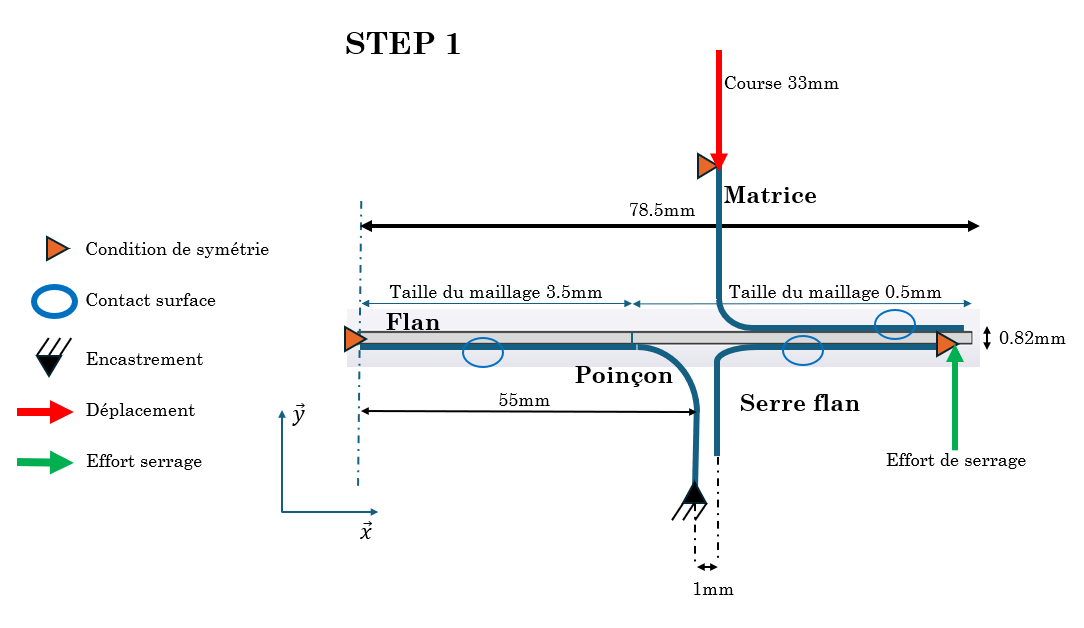
\includegraphics{FiguresALL/Methodologie/STEP1V1.png}}
        \caption{Etape 1}
        \label{fig:CL_Step1}
    \end{subfigure}
    \hfill
    \begin{subfigure}[t]{0.48\textwidth}
        \centering
        \adjustbox{width=\textwidth, height=5.5cm, keepaspectratio}{%
            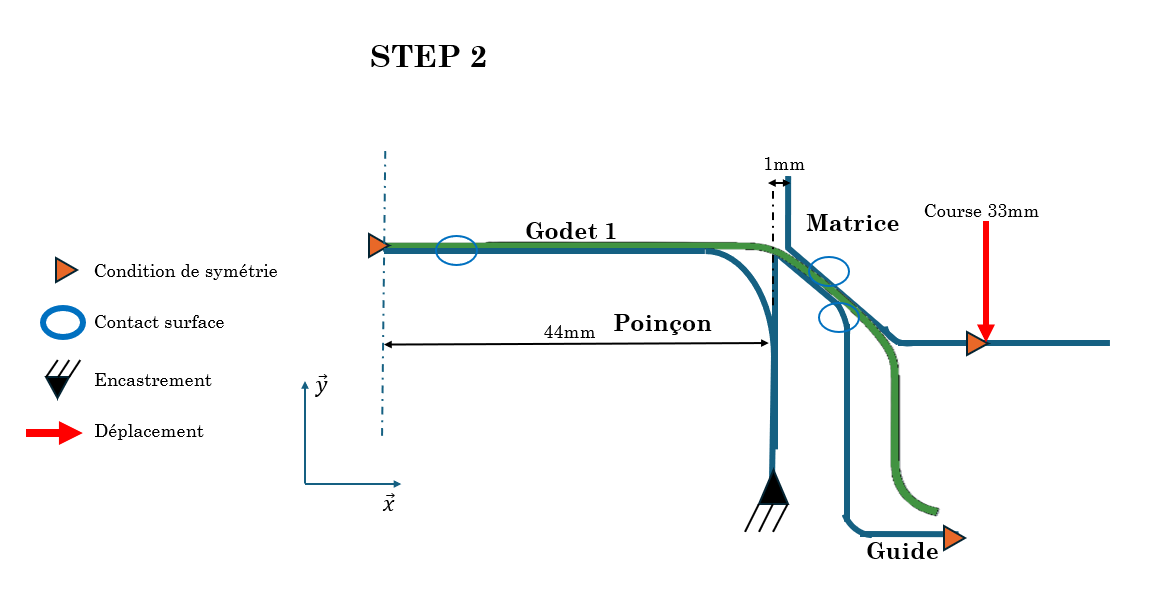
\includegraphics{FiguresALL/Methodologie/STEP2V1.png}}
        \caption{Etape 2}
        \label{fig:CL_Step2}
    \end{subfigure}
    \caption{Les interactions et conditions aux limites pour la simulation des deux étapes d'emboutissage}
    \label{fig:CL_modele}
\end{figure}
%fin figure
\subsubsection{Extraction numérique du profil du godet}
Une fois que les résultats des calculs numériques ont convergé, un programme Python a été réalisé pour extraire les profils intérieur et extérieur du godet. La méthode de post-traitement repose sur l'extraction 
des coordonnées initiales et des déplacements nodaux depuis le fichier de résultats ABAQUS (\textit{.odb}) via l'API Python 
\texttt{odbAccess} d'ABAQUS~\cite{Puri2011},. 
La position finale de chaque nœud est reconstituée par :
\begin{equation}
    \mathbf{P}_{final} = \mathbf{P}_{initial} + \mathbf{U}_{final}
    \label{eq:pos_finale}
\end{equation}
où $\mathbf{U}_{final}(U_r, U_z)$ est le vecteur de déplacement nodal extrait à l'incrément final du calcul.

%fin Méthode d'acquisition des points de profil






% --------------------------------------------------
\newpage
\section{Résultats}
% --------------------------------------------------

\subsection{Expérimental}

% Contenu à rédiger

\subsection{Simulation Numérique}

% Contenu à rédiger

% --------------------------------------------------
\section{Discussion}
% --------------------------------------------------

% Contenu à rédiger

% --------------------------------------------------
\section{Conclusion}
% --------------------------------------------------

% Contenu à rédiger

% --------------------------------------------------
%\section*{Références}
\addcontentsline{toc}{section}{Références}
% --------------------------------------------------

% Insérer ici votre bibliographie (BibTeX ou manuel)
\clearpage  % ← INDISPENSABL
\bibliographystyle{plain}
\bibliography{Biblio}

\end{document}
